% TODO: change font size to 11pt, 12pt or 13pt
\documentclass[a4paper,12pt,twoside]{book}
\usepackage[table,xcdraw]{xcolor}
\usepackage{graphicx}
\usepackage{listings}
\usepackage{listings-xml}
\usepackage{listings-json}
\usepackage{makecell}
\usepackage{float}
\usepackage{hyperref}
\usepackage[T1]{fontenc}
\usepackage{mathptmx}
\usepackage{amsmath}
\usepackage{wasysym}
\usepackage[utf8]{inputenc}
\usepackage{setspace}
% TODO: change margin to 1in, 1.5in or 2in
\usepackage[paper=a4paper,margin=1in]{geometry}
\usepackage{imakeidx}
\usepackage{tikz}
\usepackage{fancyvrb}
\usepackage{amssymb}% http://ctan.org/pkg/amssymb
\usepackage{pifont}% http://ctan.org/pkg/pifont
\usepackage{txfonts}
\newcommand{\cmark}{\ding{51}}%
\newcommand{\xmark}{\ding{55}}%
\usepackage{caption}
\usetikzlibrary{positioning, quotes}
\usepackage{csquotes}
\usepackage[english]{babel}
%%\usepackage[skip=10pt plus1pt, indent=40pt]{parskip}
\usepackage{parskip}
\usepackage{glossaries}
\usepackage[
  backend=bibtex,
  style=ieee,
  sorting=ydnt
  ]{biblatex}
\addbibresource{quotes.bib}
\makeindex

\newcommand{\putimage}[4] {
  \begin{figure}[H]
    \centering
    \includegraphics[width=#4\linewidth]{#1}
    \caption{\protect#2}\label{#3}
  \end{figure}
}

\newcommand{\putsubimage}[5] {
  \begin{minipage}{#4\linewidth}
    \centering
    \includegraphics[width=#5\linewidth]{#1}
    \caption{#2}\label{#3}
  \end{minipage}
}

\newcommand{\putimagecouple}[2] {
  \begin{figure}[!htb]
    \centering
    #1
    \hspace{0.5cm}
    #2
  \end{figure}
}

\newcommand{\putimagetriple}[3] {
  \begin{figure}[!htb]
    \centering
    #1
    #2
    #3
  \end{figure}
}

\newcommand{\putimagequadruple}[4] {
  \begin{figure}[!htb]
    \centering
    #1
    \hspace{0.5cm}
    #2
    \linebreak
    #3
    \hspace{0.5cm}
    #4
  \end{figure}
}

\newcommand{\FilledCircle} {$\CIRCLE$}%
\newcommand{\EmptyCircle}  {$\Circle$}%
\newcommand{\HalfCircle}{$\LEFTcircle$}%
\newcommand{\FineGrained}   {$\circledvee$}%
\newcommand{\CoarseGrained} {$\circledwedge$}%

\makeglossaries
\newglossaryentry{gl:transit}{name={transit}, description={Describes a group of traveling vehicles or the act of traveling through the road network.}}
\newglossaryentry{gl:traffic}{name={traffic}, description={The phenomenon of high density flows where there is the perception of being slowed down.}}
\newglossaryentry{gl:jam}{name={jam}, description={A deadlock traffic event.}}

\begin{document}
    
    \begin{titlepage}
        
        \noindent
        \begin{minipage}[t]{0.19\textwidth}
            \vspace{-4mm}{
\includegraphics[scale=1.15]{logo_unimib.pdf}}
        \end{minipage}
        \begin{minipage}[t]{0.81\textwidth}
        {
                \setstretch{1.42}
                {\textsc{Università degli Studi di Milano - Bicocca}} \\
                \textbf{Scuola di Scienze} \\
                \textbf{Dipartimento di Informatica, Sistemistica e Comunicazione} \\
                \textbf{Master Degree in Computer Science} \\
                \par
        }
        \end{minipage}
        
	\vspace{40mm}
        
	\begin{center}
            {\LARGE{
                    \setstretch{1.2}
                    \textbf{Unconventional reinforcement learning on traffic lights with SUMO}
                    \par
            }}
        \end{center}
        
        \vspace{50mm}

        \noindent
        {\large \textbf{Supervisor:} Prof. Giuseppe Vizzari}
        
        \vspace{15mm}

        \begin{flushright}
            {\large \textbf{Candidate:}} \\
            \large{Refolli Francesco} \\
            \large{Matricola 865955} 
        \end{flushright}
        
        \vspace{35mm}
        \begin{center}
            {\large{\bf Academic Year 2024-2025}}
        \end{center}

        \restoregeometry
        
    \end{titlepage}

    \begin{abstract}

This thesis investigates the effectiveness of curriculum learning approaches for modular training processes as alternative to monolithic (exhaustive) experience generation processes, compares tabular reinforcement learning methods to deep reinforcement learning models, evaluates the benefits of learning agents as opposed to fixed cycle traffic light programs, analyzing sensitivity of key hyperparameters such as the number of quantization levels for state space discretization, evaluates the advantages given by multi agent learning techniques, which involves sharing observations and rewards among agents, and finally determines whether a self-adaptive algorithm is able to update and correct the agent over time to make up for performances degrading over time due to demand and infrastructure changes.
A fork of the SUMO-RL framework, a bridge between SUMO (Simulator of Urban MObility) and Python which provides an integrated environment for developing and running reinforcement learning models, has been developed in order to answer the aforementioned research objectives,  enhancing its performance and capabilities, implementing new agents and observation/reward functions, allowing agents to share slices of observations/rewards and adding a self-adaptive algorithm for learning on degrading performances. Experiments are executed with the computational resources provided by hpc-ReGAInS@DISCo, which is a MUR Department of Excellence Project within the Department of Informatics, Systems and Communication at the University of Milan-Bicocca.

\end{abstract}

    \printindex
    \tableofcontents
    \printglossaries
    \renewcommand{\baselinestretch}{1.5}

    \chapter{Introduction}

    \chapter{Traffic Science}

\section{Introduction}

\paragraph{Terminology}

In the rest of the document we will refer to \textit{transit} or \textit{flow} to indicate a group of traveling vehicles.
The word \textit{traffic} will be used only indicate the phenomenon of high density flows where there is the perception of being slowed down.
The word \textit{jam} will indicate strictly a deadlock traffic event.

\paragraph{Vehicles}

This is a umbrella term for referring to any kind of entity which travels along a network.
Vehicles \textbf{can} have an \textit{origin} and a \textit{destination}: for example, private motor vehicles are usually driven in order to go from a \textit{point-of-interest} A to a point point-of-interest B.
An interesting exception are those public transit vehicles serving on a \textit{circle line} like the M3 City Circle Line of Copenhagen, and in general vehicles offering public transit logically have more than one destination while carrying out a trip.
Vehicles attempt to follow a \textit{desired path}, which is influenced by various factors: network knowledge, habits, transit regulations and so on.
This path can diverge from the \textit{actual path} they end up following for various reasons: accidents, infrastructure works, events and maybe illegal parking.
A notable exception are fixed route vehicles (such as public transit) and in particular track-constrained vehicles (such as trams and trains).
In both cases, the whole journey is not required to be completed: a vehicle can override its route because of change of heart (the case of private vehicles), rescheduling (the case of public transit) or else.
Depending on the goal of a simulation, the flow can be restricted to a small set of vehicle types, but in the real world, the vehicle flow can be heterogeneous: cars, trolleybuses, trams, emergency vehicles, trucks, bicycles, motorbikes and so on. Each vehicle has different physical properties and different allowances.
Vehicles allowance rules can be defined by diving the flow with respect to origin/destination, vehicle type (cars \textit{mustn't} ride in bike lanes), local regulations (in some cities, taxis \textit{may} use public transit lanes), vehicle properties (\textit{only} motor vehicles able to reach at least 60 km/h can drive on the motorway) or even driver properties (\textit{limited traffic zones} are open only for residents).
This partitioning activity is a form of transit regulation and characterizing vehicles by their properties rather than transparent objects helps (TODO: CITAZIONE) in managing their transit, resolving path conflicts and also enhancing the quality of life of residents (a bypass \textit{should} cut a significant amount of transit vehicles in city centers).

\paragraph{Infrastructure}

The road network can be represented with a \textbf{directed multi-graph} of intersections and roads. Each road has one or more lanes, a maximum speed and vehicles allowances dictating which kind of vehicles are allowed to flow through it. While more simplistic models use undirected graph with labelled edges to represent lanes and one/two-way traffic, it should be noted that a simple directed graph wouldn't be sufficient as in real-world road networks the may be more different links between an intersection. While some network slices could be represented with a single edge, there are more complex situations as in figure \ref{fig:multigraph-is-better-than-nothing} (a slice of Viale Zara, Milan, Italy) in which two big intersections are linked with two main one-way three-lane roads, two side one-way one-lane roads ("controviali") and two dedicated links for tramway vehicles. These roads are physically separated with median strips and each link may allow for different turns within the intersections. Of course, the implementation model can be optimized for performance, but the logical model should remain a multi-graph because it better represents the features of the road network.

\paragraph{Traffic}

\textbf{Traffic} can be defined as a flow of vehicles on a network with peaks of density in some locations in which the average speed of those vehicles is significantly lower than the average of the entire network.
Mathematically speaking, \textbf{traffic} emerges when many vehicles need or want to transit through a shared path which hasn't enough capacity for handling this high number of users.
Urban planning authorities have since then taken this hint quite literally, adding lanes year-by-year, but in the end the only result was an increase in the number of road vehicles with unchanged transit density or, even worse, with higher travel times \cite{Speck2018}.
In this context, \textbf{traffic science} comes in help: it seeks to understand the causes of traffic as a social \textit{phenomenon} modeling demand and analyzing flaws and strengths of infrastructure.

In the following sections I'll explain and analyze the impact of some strategies for transit regulation and traffic reduction. I'll introduce the concepts of demand modeling. Finally I'll explain the main assumptions for the present simulation and present the scenarios being used.

\section{Transit Regulation}

All the strategies presented in this section involve the usage of infrastructure artifacts in order to optimize transit. The first group aims to manage excessive flows by organizing them into different streams by origin, destination or mean of transportation and modifying the road infrastructure. The second aims to reduce route conflicts and optimize the usage of intersections. None of those is able to "fix" traffic, there are no silver bullets. This section is intended to introduce the reader to the context of transit regulation.

\subsection{Managing high flows}

\paragraph{Just one more lane}

What happens when among all the route that can be possibly be followed there is one which is faster and more convenient? Different streams are going to merge into a single huge flow which is slower than the other ones. A reasonable but ineffective action is to increase the number of lanes \ref{fig:atlanta-georgia-freeway}, but that adds only capacity to the system. It temporally fluidify traffic until other vehicles arrive into the system because it has become more convenient than their current route, and eventually traffic reemerges.

\paragraph{Bypasses, freeways, motorways}

Freeways and motorways are an example of \textit{specialized roads} which can be used to segregate the flows of vehicles needing to travel long distances from the local/regional transit. Those are generally built far from urban areas and those are what prevented urban planners from extending local roads into ten-lanes wide monsters. A further example of specialized road are bypasses, which are used to cut travel times and reduce the number of vehicles that go through the city center, but can also be used in combination with motorways. For example, in image \ref{fig:bologna-bypass} are reported three alternatives proposed by authorities to build a bypass in the Bologna's motorway node to split the flow on the basis of whether those vehicles are going to Bologna or need to reach other destinations like Firenze and Ancona. Specialized roads are generally effective in reducing travel times and represent the more convenient way for traveling mid/long distances, however they require extensive land usage and are subject to increased demand. As they essentially only add capacity to the system, it's only a matter of time before vehicle density reaches jamming levels.

\paragraph{Transit zones}

The urban area can be divided into \textit{zones} in which some vehicles can or cannot enter with various kind of rules.
\textit{Restricted traffic zones} (\textbf{ZTL}) are effectively used in city centers to block the entrance of non-resident vehicles and reduce the number of vehicles in the area. Vehicles violating this blockage are subject to a fine. If this fine is too low or if the coverage is limited, the ZTL has the same effects of a CAS.
\textit{Controlled access zones} (\textbf{CAS}) are similar but only require the payment of a toll in order to enter in the zone. An infamous example is the Area C of the city of Milan, where in order to enter it, the driver needs to buy a ticket (but some vehicles are exempts). Usually, the toll is used as a deterrent for persuading drivers to avoid central areas. Unfortunately, this measure is usually misunderstood as a way of taxing non-residents or citizens.
Finally, in \textit{Low emission zones} (\textbf{LEZ}) the only vehicles which entrance is forbidden are the ones exceeding pollution limits (e.g. by Europe emission standards). This measure is effective only in those societies where electric vehicles (EVs) and low-emission vehicles make up a small percentage of registered vehicles, because otherwise a large number of vehicles would not be affected by this regulation.
In general, the more restrictive an area is and the more area it coverts, the more it reduces traffic and wear and tear of the road network. Nonetheless, zones can also have the side effect of increasing traffic in peripheral areas or citizen rage if the restricted area is not well served by public transit, if the are no interchange parking lots outside of the area and if it's not reachable by other means, such as buses and trains.

\paragraph{Dedicated lanes}

An effective way of cutting travel times and increasing security of vehicles traveling in a mixed network (this is the case of European cities), is drawing \textit{dedicated lanes} for public transit, bikes and pedestrians. In some cities also taxis are allowed to use public transit lanes and if the number of taxis in service is high, it ends up lowering the performance of dedicated lanes. However, cities are limited in space: dedicated lanes mean cutting the number of lanes for use of private vehicles, which take up most of the spaces in urban areas. Urban planners face opposition when cutting the space allocated to cars, so it is vital that such infrastructures are enforces and designed properly in order to satisfy the transit needs of replaced vehicles.

\paragraph{One-way roads}

Where space isn't enough for two-way roads with dedicated lanes, often a good solution is the implementation of one-way roads, which also lead to safer crossings and more manageable flows. This measure actually increases travel times of vehicles, which could induce some private vehicle passengers/drivers to travel with mass public transit or by bicycle, which ultimately can decrease mean travel time of all the users of the network.

\subsection{Managing conflicts}

\paragraph{Cloverleafs}

Intersections can be built in the form of \textit{cloverleafs} to remove entirely conflicts from crossing flows. While this offer high capacity and speed, it requires excessive land usage (as can be seen in figure \ref{fig:houston-interchange-siena}) and cannot be built in urban context without erasing entire neighborhoods.

\paragraph{Precedence rule}

In urban area, non regulated intersections often follow the precedence rule: a vehicle should wait for the transit of a vehicle coming from its right, for example. The clear advantage is the lack of specialized infrastructure, at the cost of dependency on human reaction times and some times it can lead to deadlocks.

\paragraph{Roundabouts}

In roundabouts, the precedence rule is "inverted": the precedence is given to vehicles which are already in the roundabout. Depending on reaction times, it is observed that it grants a continuous flow and minimizes idle times.

\paragraph{Traffic lights}

With respect to other regulation strategies, \textit{traffic lights} are more \textbf{interesting} since they offer flexibility and regulators can apply different programs over time.

\subparagraph{Fixed cycle}

The most common program is the \textit{fixed cycle program}. Every X seconds its state changes, switching from green to yellow and red, effectively selecting from which lanes vehicles are allowed to occupy the intersection and where they can go. An intuition is that with low cycle time (e.g. 10 seconds), the intersection behaves like a roundabout, which is advantageous when dealing with incoming traffic uniformly distributed among the entrances. With long cycles, the queue is less segmented (as start-and-stop phenomenon is reduced) but depending on the distribution of the incoming flows, it can lead to a waste of time, as vehicles from a trafficked main road may need to wait on red a long cycle with a deserted side road on green.

\subparagraph{Green-wave}

Traffic lights can be \textit{synchronized} in order to obtain a so-called \textit{green-wave}, in which many adjacent traffic lights are set to green in order to grant a continuous or uninterrupted flow. This can be achieved by directly synchronizing the phase of all traffic lights or by implementing a cycle schedule allowing groups of vehicles to flow in a direction while maintaining time separation with respect to preceding vehicles and vehicles from other directions crossing the intersections.

\subparagraph{Transit signal priority}

Precedence to tram and buses can be given by detecting their proximity to the traffic light regulated intersection. This drastically reduces waiting times for public transit vehicles, which eventually could reduce the number of circulating private vehicles and thus lower traffic levels. This can be applied also to other type of public vehicles like emergency vehicles.

\section{Demand models}

This section gives an introduction to demand modeling which will be useful in further chapters to explain how demand has been simulated and how scenarios have been created.
The two subsections answer two diffent aspects of demand modeling: space and time.

\subsection{Where?}

In \textit{Origin-destination matrices} (\textbf{OD Matrix}) every cell contains a number representing the approximate demand of transit vehicles from a zone A to a zone B. Depending of the scale of the simulation, zones can be regions, provinces, cities or urban districts.
For example, the Lombardy region yearly analyze traffic and demand \cite{ODLombardia2014} between its cities in order to plan maintenance and improvements in its regional road network.
It is useful that zones partition the area of interest without intersections, otherwise data could be distorted. This is often the case of urban contexts: for example Agenzia Mobilita' Ambiente e Territorio of Milan (AMAT) in 2010 \cite{ODMilano2010} had modeled the urban transit demand of the city of Milan but the zones used for OD matrix are not clearly distinguished (it can be seen in \ref{fig:odzones-milano-2010}) and therefore the matrix has to be taken with coarse-grain granularity.
Nonetheless, counting vehicles and inferring their origin destination it not an easy activity \cite{bell1983estimation}.

\subsection{When?}

Usually, mobility agencies create more than one OD matrix in order to capture how traffic levels change during a day.
Some agencies such as AMAT use three time ranges: 07:00-10:00 (morning peak), 10:00-16:00 (off-peak) and 16:00-20:00 (evening peak). 
While other entities like Regione Lombardia, provide hourly data.
In figures \ref{fig:odmatrix-milano-2010} and \ref{fig:odmatrix-lombardy-2014}, mean traffic levels from OD matrices of Milan and Lombardy region can be seen as they estimate a similar situation.
What happens during working days is that there are two major peaks, one in the morning and one in the afternoon/evening, which correspond to workers going and returning from work.
Recently it has emerged also another phenomenon called \textit{third rush hour}, which is the peak during midday due to trips with private vehicles in order to have lunch.
%% Creare un sketch grafico di come si comporta il traffico, magari da sovrapporre a quelli

\section{Settings and assumptions}

% Assumptions
%% Only cars
%% Two peak rush hours
%% Synthetic data
%% Artificial queues
%% Baseline traffic lights are using green-wave mode of operation
% Settings
%% Breda
%% Celoria

\section{Figures}

\begin{figure}[h]
    \centering
    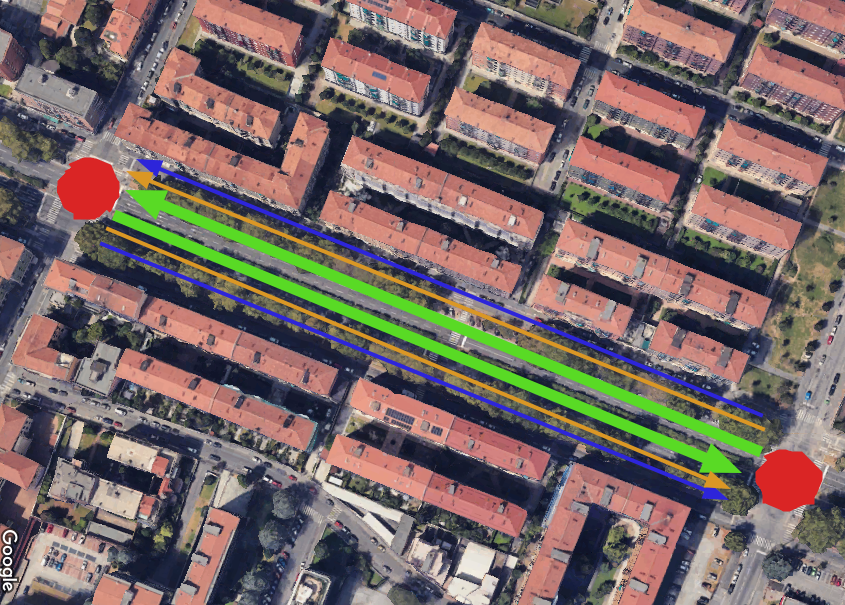
\includegraphics[width=0.75\linewidth]{figures/multigraph-is-better-than-nothing.png}
    \caption{A complex intersection pair which is connected with more different roads (Viale Zara. Milan. Italy). In \textit{green} the main lanes, in \textit{blue} the side lanes, in \textit{orange} the tramway. Source: Google Maps (2025)}
    \label{fig:multigraph-is-better-than-nothing}
\end{figure}

\begin{figure}[h]
    \centering
    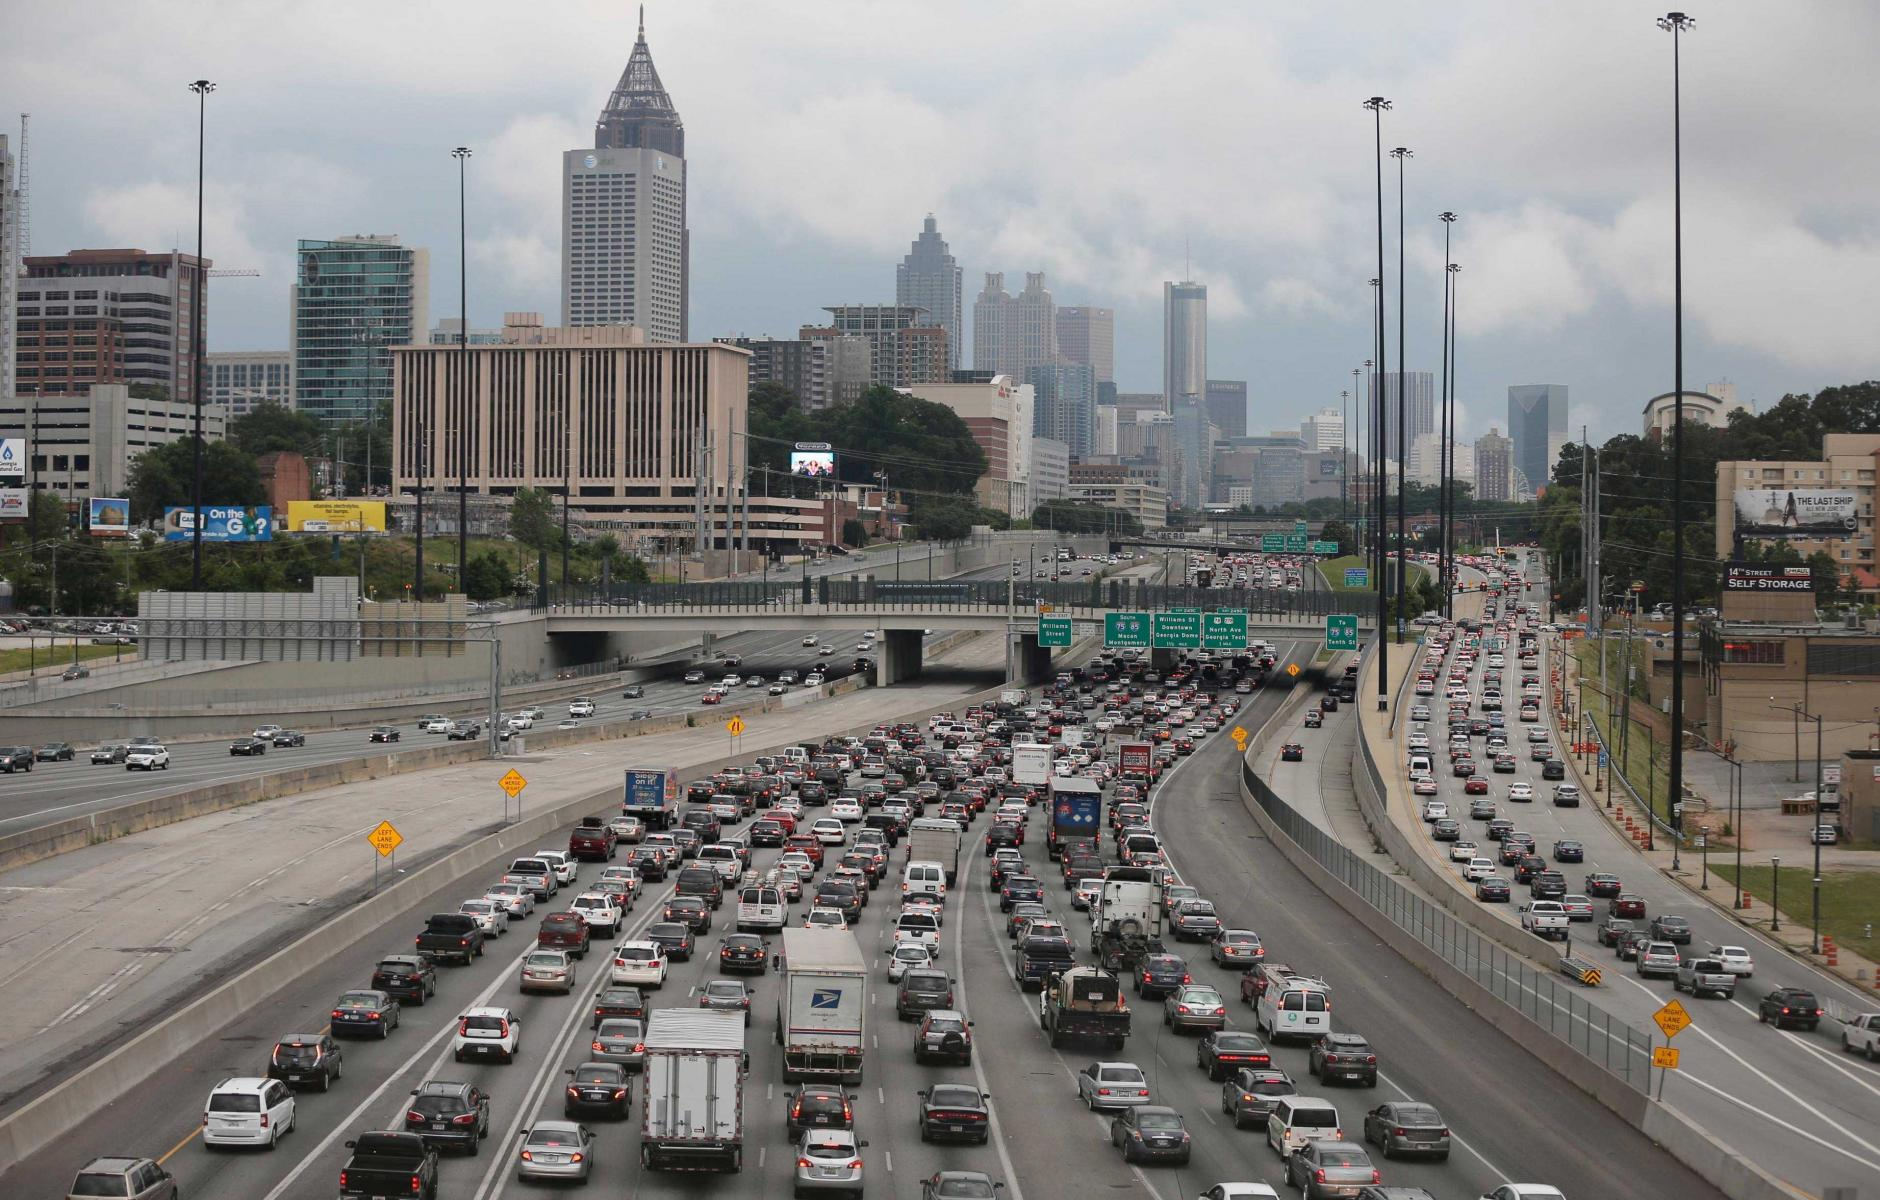
\includegraphics[width=0.75\linewidth]{figures/atlanta-georgia-freeway.jpg}
    \caption{A view of Atlanta Freeway, Georgia. Source: \href{https://www.cnu.org/publicsquare/2017/08/03/why-urban-freeway-expansion-futile}{cnu.org}}
    \label{fig:atlanta-georgia-freeway}
\end{figure}

\begin{figure}[h]
    \centering
    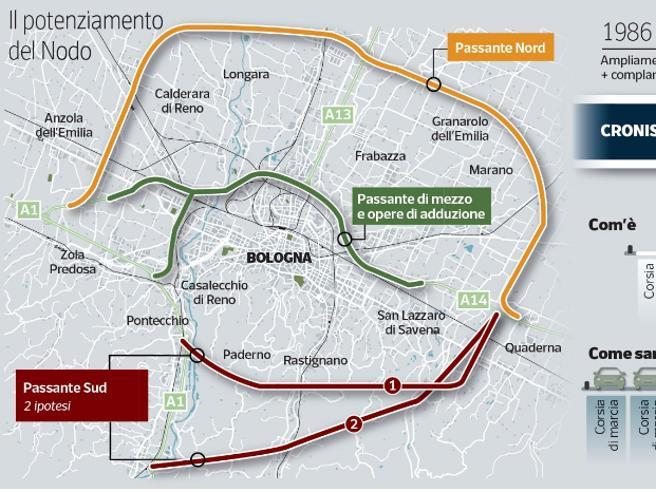
\includegraphics[width=0.75\linewidth]{figures/bologna-bypass.jpg}
    \caption{Highlight of alternatives for the Bologna node bypass. Source: Corriere della Sera}
    \label{fig:bologna-bypass}
\end{figure}

\begin{figure}[h]
    \centering
    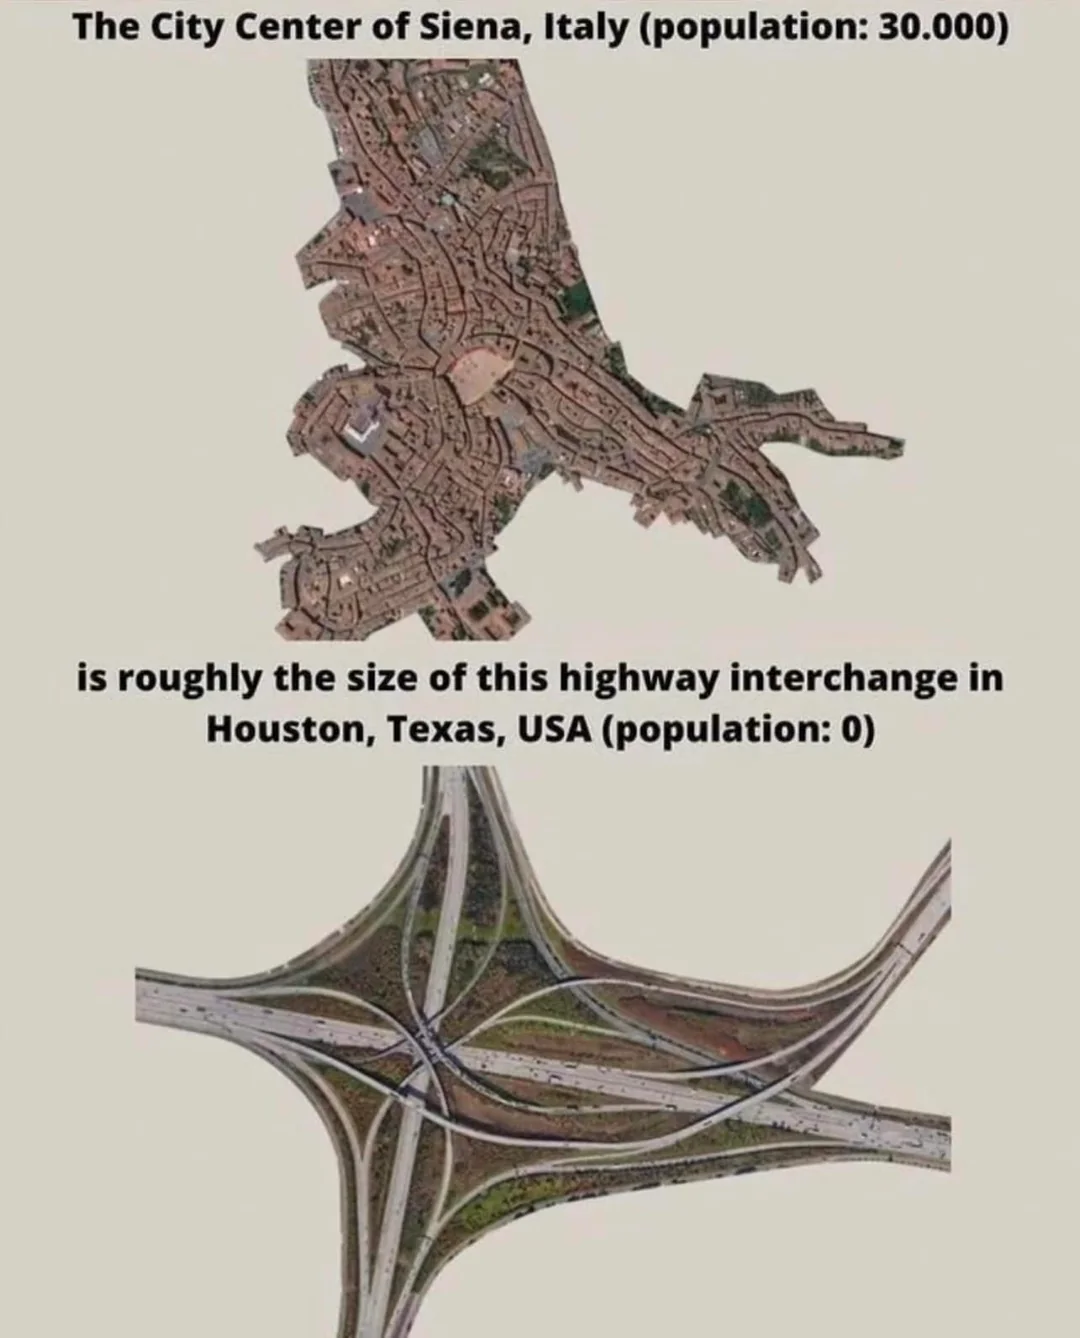
\includegraphics[width=0.75\linewidth]{figures/houston-interchange-siena.png}
    \caption{Comparison between a cloverleaf in Houston, USA, and the city center of Siena, Italy. Source: \href{https://www.reddit.com/r/geography/comments/193ryy5/siena_compared_to_highway_interchange_in_houston/}{r/geography}}
    \label{fig:houston-interchange-siena}
\end{figure}

\begin{figure}[h]
    \centering
    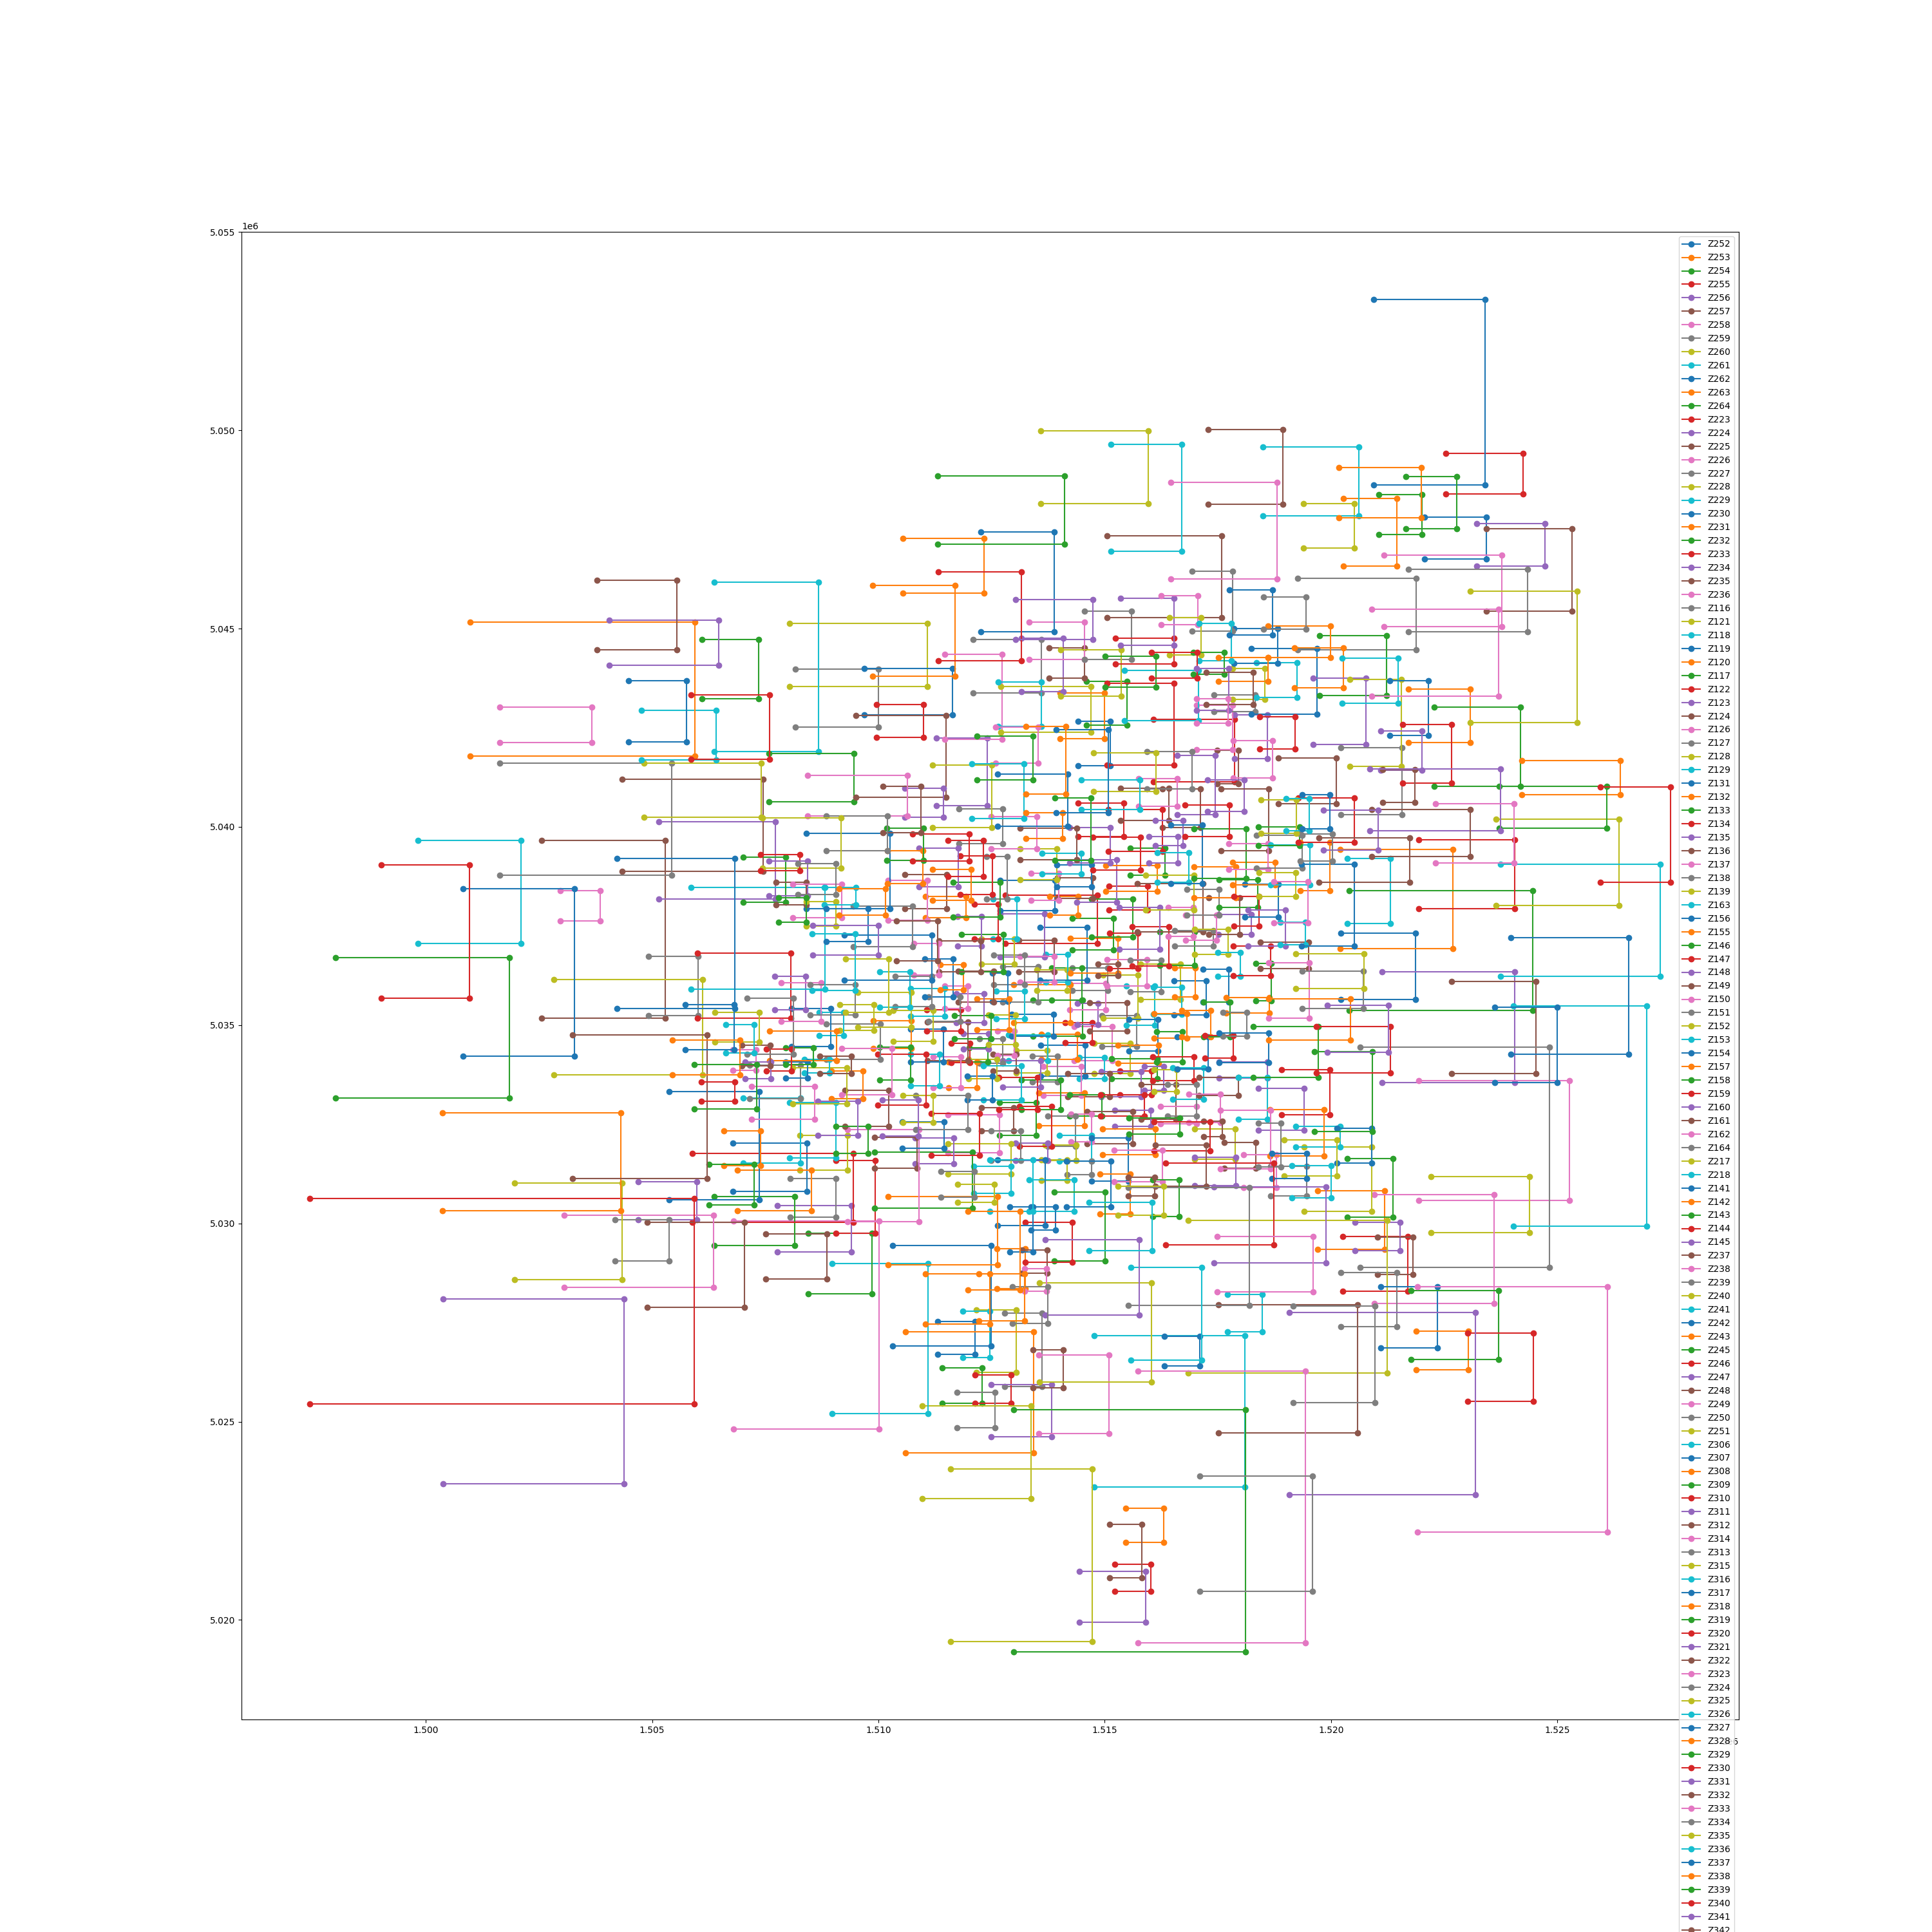
\includegraphics[width=0.75\linewidth]{figures/ODZones.Show.Milano2010.png}
    \caption{OD Zones used within the 2010 Milano AMAT model}
    \label{fig:odzones-milano-2010}
\end{figure}

\begin{figure}[h]
    \centering
    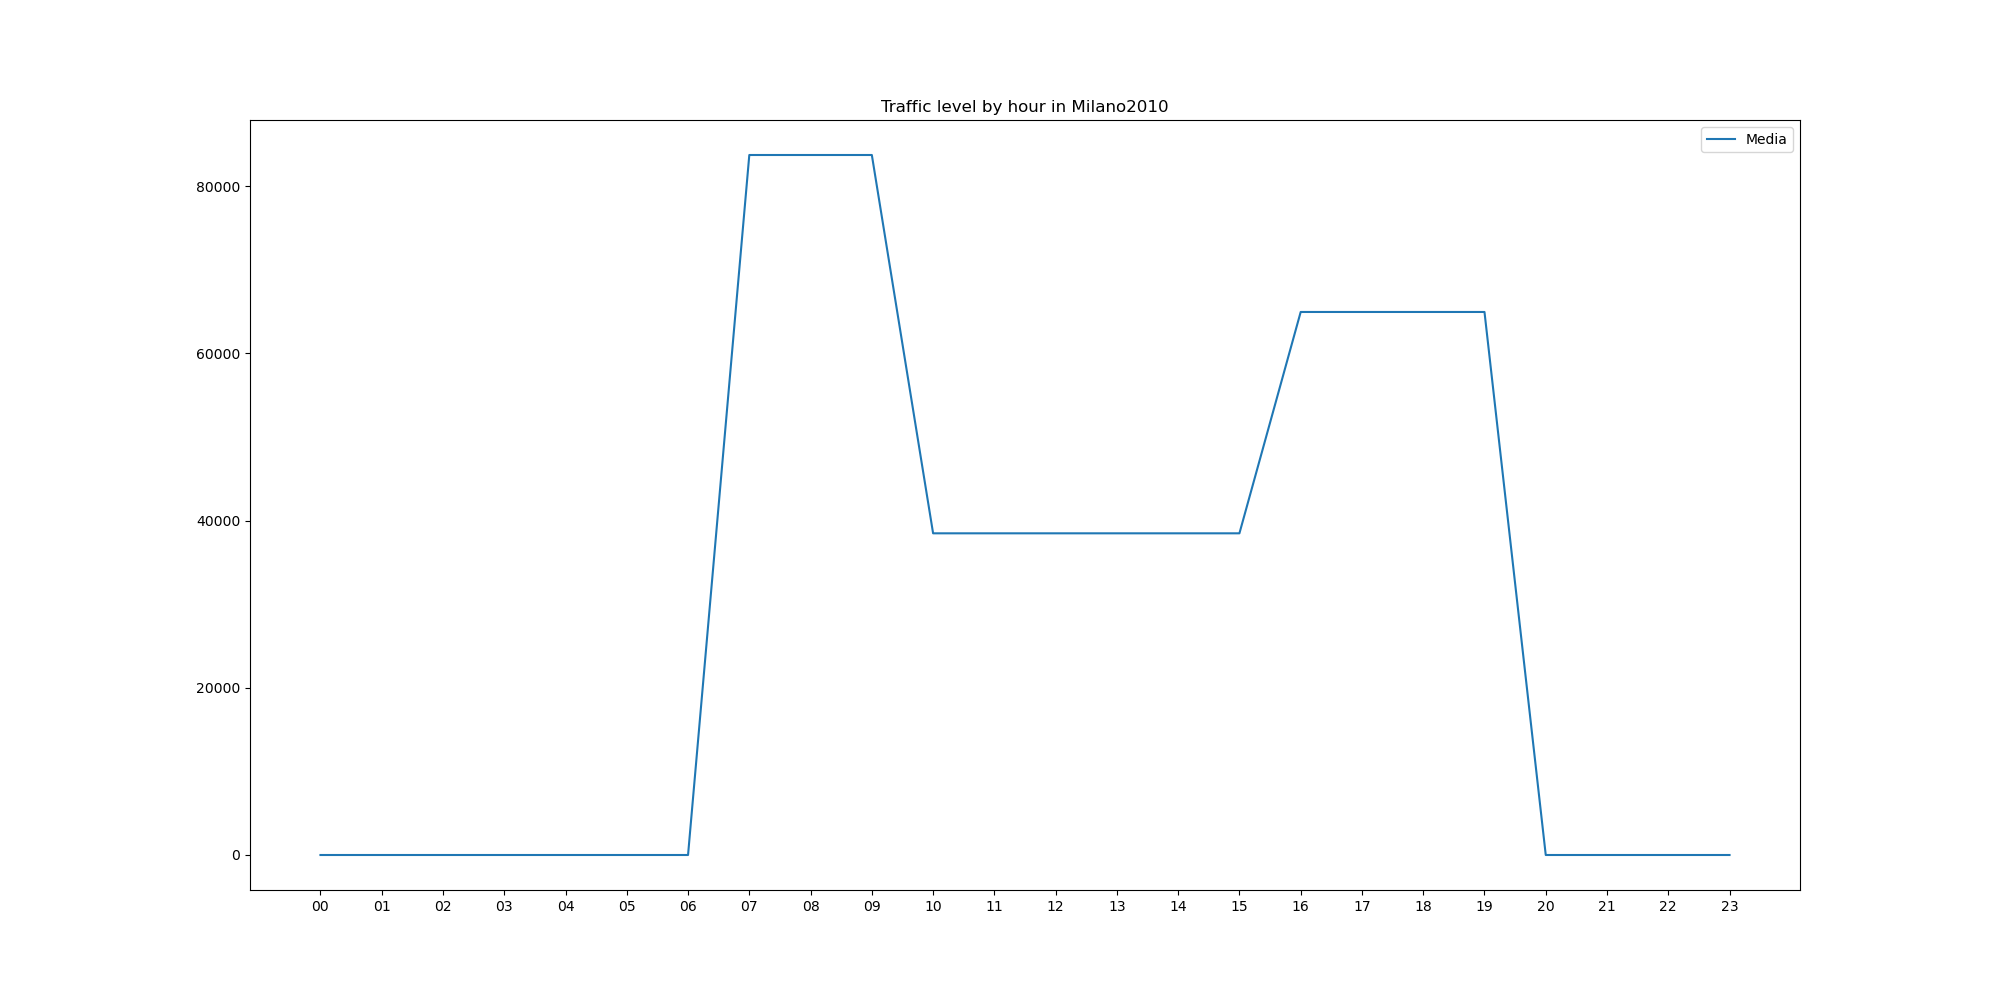
\includegraphics[width=0.75\linewidth]{figures/ODGraph.Mean.Milano2010.png}
    \caption{Traffic levels from OD Matrix of Milan in 2010}
    \label{fig:odmatrix-milano-2010}
\end{figure}

\begin{figure}[h]
    \centering
    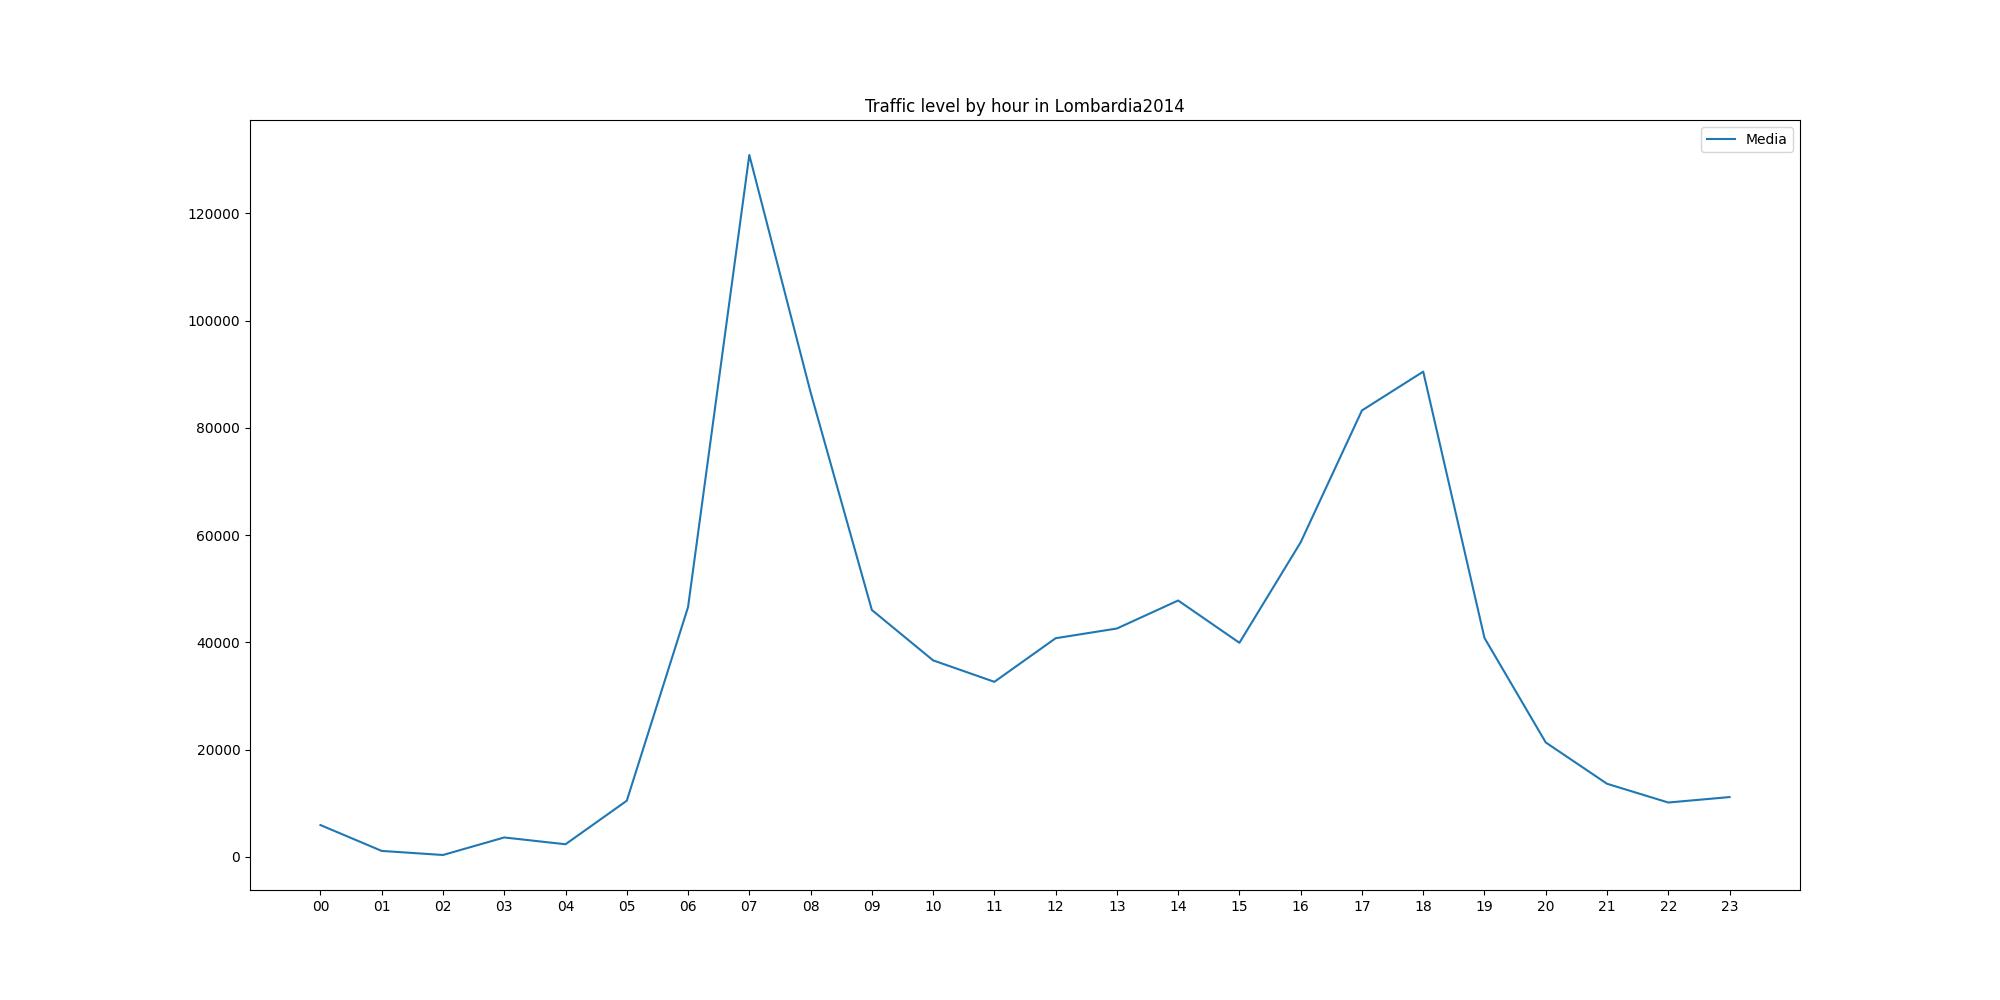
\includegraphics[width=0.75\linewidth]{figures/ODGraph.Mean.Lombardia2014.png}
    \caption{Traffic levels from OD Matrix of Lombardy in 2014}
    \label{fig:odmatrix-lombardy-2014}
\end{figure}

    \chapter{Traffic Simulations}

\section{SUMO}

SUMO (Simulation of Urban MObility) is an open source multi-modal, microscopic traffic simulator developed by the Institute of Transportation Systems at the German Aerospace Center. It accept a network description file ($*.net.xml$), a demand and flows description file ($*.rou.xml$). It comes with several utilities which enable the user to construct or edit a network or a simulation, generate demand from OD matrices, verify correctness of description files, dump slices of OpenStreetMap and more. The simulator can run headless or within a graphical user interface (which can be seen in figure \ref{fig:sumo-gui}), which let the user inspect details of network elements or vehicles at runtime and modify parameters at-fly. The user can also stop and resume the simulation as well as export its instant dump or change the simulation step.

\putimage{figures/sumo-gui.png}{A view of SUMO simulator GUI interface loaded with a simulation scenario. The picture is centered over a few intersections in which the phases of traffic lights are highlighted.}{fig:sumo-gui}{1.0}

\paragraph{TraCI}

Since the simulator has been thought as a standalone executable, there is not library to interact with and all has to be done with TraCI, a network application protocol defined as part of the SUMO project. Queries can be used to obtain data from the simulation, such as vehicles position, speed and route, lane density, traffic lights programs and state. A notable limitation is that there is no clear granularity for retrievable content. For example, it is possible to ask the \textit{mean waiting time of vehicles in a specific lane} but not the \textit{mean accumulated waiting time of vehicles of that lane}. The reason? Not a clue. Nonetheless, you may need to ask single informations a query at a time, which is rather slow. For that reason, I recommend to cache and compute "manually" data whenever it is possible in order to avoid costly network connections. Ten queries per vehicle or per lane don't sound a lot until one discovers to have twenty-five thousand vehicles and a hundred lanes per simulation step just for a simple five intersection scenario. In further chapters I will explain which metrics I track, what they represent and why I need them. TraCI also allows to \textbf{set} some data, such as traffic light program and current state. This is important for implementing traffic light agents on top of SUMO. In further sections I will introduce the concept of multi agent simulation and how a traffic light can be seen as a proper agent.

\paragraph{Netedit}

SUMO has a scenario creation utility which enables the user to build and edit a network as well as demands and other additional data.
In figure \ref{fig:netedit-network}, the graphical interface for shaping a network can be seen. It allows to create junctions and edges, editing intersection connections, adding traffic lights and TAZ and more.
In figure \ref{fig:netedit-demand}, the graphical interface for adding demands can be seen. It allows to create routes, single vehicle trips, vehicle flows and more options to edit vehicle types and more.

\putimage{figures/netedit-network.png}{A view of SUMO Net-edit utility. This mode enables the user to modify the network of the simulation.}{fig:netedit-network}{1.0}
\putimage{figures/netedit-demand.png}{A view of SUMO Net-edit utility. This mode enables the user to modify the transit demand of the simulation.}{fig:netedit-demand}{1.0}

\paragraph{Network}

% Edges
SUMO transport networks are mainly composed of edges and intersections. An \textbf{edge} is defined with a \textit{source} and a \textit{sink} intersection, it has a \textit{priority} and a \textit{type}, which declares the edge role within the network. \textit{Normal} edges represents real roads, while \textit{internal} edges are an abstraction used within intersections to configure where an incoming vehicle can go to. This last concept will be explained better when talking about intersections. There are also \textit{crossing} and \textit{walkingarea} edges, which are useful when dealing with simulations involving an active role of pedestrians. Each edge contains more \textit{lanes}.

% Lanes
Each lane defines its \textit{shape} as a sequence of coordinates (must be enabled via parameter $customShape$), its maximum \textit{speed} in meters per second, its logical length and its set of \textit{allowed} or \textit{disallowed} vehicles (as can be seen in figure \ref{fig:netedit-allowances}). More will be said about vehicle types later on, but for now it suffices to say that this option is used to create bike lanes, tram ways and so on. Each lane also declares its ordinal \textit{index} with respect to its edge, which is useful when declaring connections between roads, junctions and lanes.

\putimage{figures/netedit-allowances.png}{A view of SUMO Net-edit utility. Setting allowances is possible with a dedicated panel on lanes and edges}{fig:netedit-allowances}{0.5}

% Intersections
Junctions are the nodes of the SUMO multi graph, and represent intersections (default) as well as other types of nodes. For example, a \textit{deadend} junction is used to represent an entry/exit point of the simulation. There are also \textit{internal} junctions which define a waiting position within the intersection. A junction has some \textit{incoming lanes} and some \textit{internal lanes}. The internal lanes, mentioned before, a the joints within the intersection which link an incoming lane with an internal edge and then an internal edge with an outcoming lane. Internal connections are highly customizable, as can be seen in figure \ref{fig:netedit-internal-connections}, in which left turns are forbidden entirely (as happens in real main roads like Viale Monza).

\putimage{figures/netedit-internal-connections.png}{A view of SUMO Net-edit utility. The (editable) internal connections of an intersection are highlighted. In blue the selected lane, in green the enabled turns, in yellow the lanes which SUMO suggests not to enable to avoid directional conflicts.}{fig:netedit-internal-connections}{0.5}

% Traffic Lights (and programs)
By default, intersections are regulated with the precedence rule, but traffic lights may be created in order to optimize the transit. A traffic light has one or more programs but has exacly one active program. A program is a sequence of states which will be hold for a fixed amount of time before changing to the next one (repeated cyclically). A state is declared as a string of characters ("\textbf{r}" for \textit{red}, "\textbf{y}" for \textit{yellow}, "\textbf{g}" for \textit{green} and "\textbf{G}" for \textit{priority green}), one for each connection. It is strongly recommended to mix \textit{green} (G) and \textit{priority green} (G) in order to avoid deadlocks and reduce unrealistic conflicts. For example, in figure \ref{fig:netedit-tllogic} is shown an intersection in which straight and right directions are prioritized over left turns. Recalling what has been said about internal edges, a connection links an incoming lane and an outcoming lane in order to allow or disallow transits and turns. All the declared connections which are subject to a traffic light program are indexed with the ordinal parameter \textit{linkIndex}. This form of representation allows the user to reproduce any realistic scenario.

\putimage{figures/netedit-tllogic.png}{A view of SUMO Net-edit utility. The (editable) program of a traffic light is highlighted.}{fig:netedit-tllogic}{0.5}

% Roundabouts
Intersections can also be regulated with roundabout, which can be created via SUMO Net-edit utility as can be seen in figure \ref{fig:netedit-roundabout}. These are not \textit{real} roundabouts, just a crooked representation of how a roundabout works. It sets some waiting positions inside a junction agglomerate in order to reproduce the cyclic behavior of vehicles in roundabout.
Interestingly, since those are created by blending more virtual junctions, one can have SUMO to add traffic lights to roundabout waiting positions, with questionable results.

\putimage{figures/netedit-roundabout.png}{A view of SUMO Net-edit utility. SUMO also supports simulation of roundabout, but are coerced into crooked intersections.}{fig:netedit-roundabout}{0.5}

\paragraph{Demands}

Demands is expressed in terms of vehicles trips or vehicles flows. For more realistic scenarios, it is recommended to use the first option if an exact timeline of vehicles is available or if one is testing a specific situation that could happen inside inside a network slice. For example, GTFS data can be used to reproduce one-to-one the behavior of a public service network. An important notice is that the actual demands implementation is then randomized by SUMO via its simulation seed, so in order to be reproducible one should hold a specific seed.

Both trips and flows declare a used vehicle type, which is the kind of entity generated into the simulation at runtime. As can be seen in figure \ref{fig:netedit-allowances}, SUMO supports a large variety of vehicles types. Depending on the simulation aims, is it possible to include private vehicles such as \textit{cars} (there is also a distinction between internal combustion engines and electric vehicles), \textit{motorbikes}, \textit{trucks}, \textit{bicycles} but also \textit{pedestrians} and \textit{wheelchairs}. The choice for public service and non-road vehicles is wider: emergency vehicles like \textit{ambulances}, road public transit like \textit{taxis}, \textit{urban} and \textit{suburban buses}, railway vehicles such as \textit{trams}, \textit{light rail}, \textit{heavy rail} (with the distinction between electric/non-electric convoys), airborne vehicles such as \textit{airplanes} and \textit{drones}, special duty vehicles such as government/police/army vehicles and finally \textit{ships}. 

Vehicles generated by trips and flows follow a route which can be statically allocated or change dynamically during the simulation. The SUMO simulator will check if those declared routes are continuous and valid before even starting the simulation: when using utilities other than Net-edit or other SUMO related software, the user must ensure that routes were generated correctly. There is also a specialized SUMO tool which checks routes correctness.

Inside the demands description file, a static route must be declared as a continuous sequence of waypoints (the "via" attribute, which can contain only edges). The Net-edit utility is very helpful because it lets the user to set a discontinuous sequence of waypoints and will use a routing algorithm in order to complete the selected route. For example, in figure \ref{fig:netedit-trip-between-edges} I selected an edge in the bottom left corner and an edge in the top right corner. Enforcing the connection links defined in intersections and the lane vehicle type allowances, it has found an optimal \textit{valid} route between those waypoints. Net-edit also warns the user about unreachable edges for the current route, as can be seen in figure \ref{fig:netedit-unreachable-edges}, where those edges are highlighted in pink.

\putimage{figures/netedit-trip-between-edges}{A route from edge-to-edge, completed automatically by Net-edit.}{fig:netedit-trip-between-edges}{0.5}
\putimage{figures/netedit-unreachable-edges.png}{Net-edit highlights in pink the unreachable edges for the current route.}{fig:netedit-unreachable-edges}{0.5}

Dynamic routes can instead be declared simply by stating an origin and a destination waypoint. One can create routes this way with edges, junctions and TAZs. At runtime, SUMO will generate a concrete route for those vehicles, which can be randomized and changed even during the trip execution if specified. It is important to notice that routes can also be defined independently from trips and flows: when creating such trips and flows, they can be simply attached to already declared routes.

I previously talked about junctions and edges in SUMO networks, but what are TAZs? Recalling what has been said in the last chapter about \textit{OD matrices}, the transport network can be divided into (maybe intersecting) zones containing junctions and edges. If a route is defined over TAZs as waypoints, the resulting vehicles will appear on edges covered/crossed by the origin TAZ and will be routed against an edge covered/crossed by the destination TAZ. The same happens for intermediate TAZ waypoints. This allows to recreate realistically demands described by OD matrices. For example, in figure \ref{fig:netedit-trip-between-tazs} I defined a route from a TAZ in the bottom left corner to a TAZ in the top right corner.

\putimage{figures/netedit-trip-between-tazs.png}{Trips can be created between TAZs.}{fig:netedit-trip-between-tazs}{0.5}

Once that vehicle types and routes are set, there are other options which can be used to customize the journeys. One can define the departure/arrival speed, lane, position. For example, the departure lane can be either set to \textit{free} (depart from a random available lane) or from a specified lane. This can create custom scenarios where vehicles can appear or disappear only at specified conditions. There also graphical options such as the vehicle color and logical options which can influence the simulation, like the number of vehicle occupants/passengers.

\paragraph{Flexibility}

% Explain general sumo-wide options
%% Acceleration model
%% Entering delays
%% Lane change granularity
%% Usage of junctions as TAZ
%% Simulation step
%% Deadlocks and recover (--ignore-junction-blocker)

\section{Multi-agent simulations}

% Concept of Multi Agent Simulations
% Agents of this simulation
%% Vehicles as agents
%%% Chaning lane is an action
%%% Driving is an action
%% Traffic light is an agent
%%% Changing to other phases is its action
%%% Its phase is its state
%%% Incoming vehicles and lanes are its observation
%% Learning agents

\section{A control plane of SUMO agents}

% Enabling device for simulation with traffic light agents
% Blends reinforcement learning into agents
% Gather metrics from vehicles and lanes in order
% Plots metrics
% Generates flows
% Executes simulations

    \chapter{Background on Reinforcement Learning}

This chapter introduces the concept of Reinforcement Learning, along with its differences from traditional machine learning approaches, its advantages and disadvantages, and its mathematical foundation.

\section{A new perspective}

Machine Learning (ML) is a branch of Artificial Intelligence concerning all those statistical techniques and algorithms that can be used to learn a task from an existing data and generalize this knowledge to unseen data. Depending on how the agents learns and what task it learns, ML can be divided into three paradigms: supervised, unsupervised and reinforcement learning.

\paragraph{Learning by example}

Supervised learning (SL) is perhaps the most intuitive and widely used learning paradigm.
The agent is given an input and returns an output. Its output is then compared with the expected output (provided along with the input) using a \textit{Loss Function}, which measures the error between the two values.
This loss is then used to update the agent's model in order to improve its accuracy.
Since the quality of the agent is defined by the similitude between its output and the reference (``correct'') output, it is essentially learning to replicate a behaviour of which the labelled dataset is an example.

Despite its simplicity, this paradigm take two strong assumptions.
1) The current output of the agent doesn't influence the goodness of a future output. That is to say: each decision or value emitted from the agent is independent temporally from other values emitted over time.
Tasks involving classification or labelling, such as identifying the class of a dry bean or spam detection, fall naturally into this category.
2) A dataset of input-output pairs is available and, more importantly, a correct output value exists and it is priorly known or computable. This restriction automatically excludes all problems involving uncertainty, long-term consequences, or scenarios in which the optimal decision depends on a sequence of past and future actions. However, it accommodates a lot of problems for which knowledge about past is available, as in prediction tasks like stock forecasting and language models.

\paragraph{Learning by inference}

Unsupervised learning (US) removes the need of labelled data, as the goal here is not to imitate known outcomes but to find hidden structure within the data itself.
Usually, this activity involves partitioning the input dataset into k classes, which result can be then applied to further processing.
Although the ultimate goal is to ensure that items within the same group resemble each other more than they resemble those in other groups, different approaches to achieve such partitioning exist, ranging from distance-based algorithms (such as K-Means) to hashing-based algorithms (such as Locality Sensitive Hashing).
In both cases, the agent is inferring an hidden connection between elements of the dataset using its features.
However, it should be noted that the resulting classification carries no semantic beyond element similarity and, in particular, there is no concept as intrinsic partitioning correctness. Which means that US cannot be applied directly in decision making problems and can only be used for aggregation tasks such as ancestral reconstruction (useful in phylogenetics) and feature extraction.

\paragraph{Learning by experience}

A useful analogy comes from early human development. Consider a toddler learning to walk. The parent may encourage the child by standing across the room and using gestures or facial expressions (such as smiles or glares) to signal success or failure. The toddler does not receive explicit instructions or labelled examples of correct foot placement. Instead, learning unfolds through trial and error, with the child gradually discovering which patterns of movement lead to praise or comfort. Reinforcement learning (RL) mirrors this process: knowledge is acquired not through imitation or discovery of structure, but through experience and consequence.

The agent is acknowledged to lie into an environment, which has an internal logic and an internal state but those are not exposed to the agent.
The agent can only observe the environment with an \textit{Observation Function}, which returns a partial view (``observation'') of its state.
This observation is then used by the agent's decision-making process (``policy'') to take an action.
The environment updates its state with a \textit{Transition Function} which applies the effects of the agent's action to the current state and computes the next state.
The agent then collects the new observation and the reward released by the \textit{Reward Function} in order to improve its action.

Therefore, instead of learning from a static dataset, the agent learns by the experience gained when interacting with the environment.
Another key intuition is that the focus of RL is not on the single action, but on the outcome of a sequence of interactions. Thus, the agents aims to maximize the cumulative reward.
For that reason, RL is applicable in all those tasks in which the quality of an action is defined also by past and future actions, such as traffic light management.

\section{Mathematics}

\subsection{Markov Chains}

The evolution of RL environment could be roughly described as a \textbf{Markov Chain}, which is is a tuple $MC = (S, P)$ where $S$ is the set of all states and $P$ is a transition function such that $P(S_n | S_{n-1})$ denotes the probability of the state $S_n$ happening given that the previous state is $S_{n-1}$. An example of Markov chain is shown in figure \ref{fig:markov-chain}. Intuitively, any episode of an environment is a sequence of states and there is some kind of transition function which moves the environment from one state to another.

Notably, an important property of Markov Chains is that \textit{past and future are mutually independent}. This may sound like a contradiction to the concept of Markov Chain, but it is in fact a simplification over statistics which allows to model an environment more easily. The appearance of the current state is assumed to be influenced only by the appearance of the previous state. This principle can be summarized as $P(S_n | S_{n-1}) = P(S_n | S_{n-1}, S_{n-2}, S_{n-3}, S_{n-4})$.

Markov chains are a powerful tool for modelling stochastic environments, such as weather conditions. Supposing to have a dataset of daily weather (sunny, cloudy, rain, thunderstorm), one could compute an approximation of $P(S_n | S_{n-1})$ and use it for weather forecasting.

Now, recalling the Markov property and seeing this implementation, a valid argument against this practise of course could be that one precedent weather record isn't enough for predicting future records with sufficient accuracy. But states can also be aggregate or complex objects: Markov chains allow defining a state as the previous k records of weather data.

A more subtle detail resides in what it actually models: a Markov chain doesn't take into account the \textit{external forces} (agents' actions). For example, whether or not the Government decides to start \textit{cloud seeding} is already a game changer variable which radically changes the weather model.

\putimage{figures/markov-chain.png}{An example of three state Markov Chain}{fig:markov-chain}{0.5}

\subsection{Markov Decision Processes}

A \textbf{Markov Decision Process} is defined a tuple $MDP = (S, A, P, R)$ where S is the set of all states, $A$ is the set of all actions, $P$ is a transition function such that $P(S_n | S_{n-1}, a)$ denotes the probability of the state $S_n$ happening given that the previous state is $S_{n-1}$ with the action $a$, and $R$ is a reward function such that $R(S_{n-1}, a, S_{n})$ denotes the immediate reward of the transition from state $S_{n-1}$ to state $S_n$ with the action $a$. An example of MDP is shown in figure \ref{fig:markov-decision-process}.

This model not only accounts for agents' actions, but also provides an abstraction for expressing the quality of an action or the desirability of a certain state transition.

\putimage{figures/markov-decision-process.png}{The expansion of the Markov Chain of figure \ref{fig:markov-chain} as a Markov Decision Process. Green transitions release a positive reward, red transitions release a negative one.}{fig:markov-decision-process}{0.5}

\subsection{Policies}

The agent behaviour in a MDP environment can be defined with a \textbf{policy} $\pi$, which is a deterministic or stochastic mapping from the state set to the action set.
A deterministic policy $\pi_{det}$ is a function $\pi_{det} \; : \; S \rightarrow A$, while a stochastic policy $\pi_{sto}$ is a function $\pi _ {S} \; : \; S \times A \rightarrow [0, 1]$, denoted as $\pi _ {S}(a | s)$, where $\sum_{a \in A} \pi _ {sto} (s, a) = 1$.

The behaviour of an agent can then be evaluated by evaluating its policy: a policy $\pi _ a$ is \textit{better} than a policy $\pi _ b$ if the accumulated reward over time of $\pi _ a$ is higher than the one of $\pi _ b$.
In particular, a policy $\pi _ o$ is defined \textit{optimal} if $\forall \pi _ i \neq \pi _ o$, it holds that $\pi _o $ is \textit{better} than $\pi _ i$.
If the relative quality of a policy if defined by a scalar value, how can the accumulated rewards be computed?

\subsection{Value Functions}

\paragraph{State-value function}
\label{par:state-value-function}

The \textbf{state-value} function $V^{\pi}(s)$ evaluates the amount of expected reward obtained by following a policy $\pi$ from the state $s$.
Since both the environment and the agent's policy can be stochastic, an abstract formula to compute this concept reuses the expected value operator $\mathbb{E}$ from probability theory.
An slice of the episode of an MDP can be represented as a process graph starting from a node $s_i$, developing into a chain of states and actions. The value of this computation is given by a weighted sum of the rewards of tis transitions.
Since the same node and action can lead to different nodes, the process becomes a sequential, ramified structure as all possible transitions are recursively considered.
The expected reward of the state $s_i$ can be thought as the weighted sum of rewards of the average path along this ramified process, which leads to the following formula:

\begin{equation} \label{eq:v-pi-E}
V^\pi(s) = \mathbb{E} \left[ \sum_{t=0}^{\infty} \gamma^t R(s_t, a_t, s_{t + 1}) \mid s_0 = s \right]
\end{equation}

Here, \textbf{$\gamma$} is discount factor used for weighting the sum of gained rewards. If $0 < \gamma < 1$, then $lim ^ {t \rightarrow +\infty} \gamma ^ t = 0$ and the immediate rewards have priority over long-term rewards. Otherwise, if $\gamma > 1$, then $lim ^ {t \rightarrow +\infty} \gamma ^ t = +\infty$ and the long-term rewards have priority over immediate rewards. The value of $\gamma$ should reflect the desirability of state transitions and the end goal of the agent learning in this environment. For this reason, it may also be the case for $\gamma = 1$ if immediate rewards and long-term rewards have the same importance in defining the goodness of the agent behaviour. For practical reasons, the abstract $V^{\pi}(s)$ formula can be rewritten to a more manageable recursive form:

\begin{equation} \label{eq:v-pi-bellman}
V^{\pi}(s) = \sum _ {a \in A} \pi (a | s) \sum _ {s' \in S} P(s' | s, a) \left[ R(s, a, s') + \gamma V^{\pi}(s') \right]
\end{equation}

\paragraph{Action-value function}
\label{par:action-value-function}

The \textbf{action-value} function $Q^{\pi}(s, a)$ evaluates the amount of expected reward obtained by following a policy $\pi$ from the state $s$ using the action $a$.
Reusing the reasoning of Subsection \ref{par:state-value-function}, the abstract formula can be written as:

\begin{equation} \label{eq:Q-pi-E}
Q^\pi(s, a) = \mathbb{E} \left[ \sum_{t=0}^{\infty} \gamma^t R(s_t, a_t, s_{t+1}) \mid s_0 = s, a_0 = a \right]
\end{equation}

Again, for practical reasons, the abstract $Q^{\pi}(s, a)$ formula can be rewritten to a more manageable recursive form:

\begin{equation} \label{eq:Q-pi-bellman}
Q^{\pi}(s, a) = \sum _ {s' \in S} P(s' | s, a) \left[ R(s, a, s') + \gamma \sum _ {a' \in A} \pi (a' | s') Q^{\pi}(s', a') \right]
\end{equation}

\paragraph{Usefulness of value functions}

Both the \textit{state-value} function $V^{\pi}(s)$ \ref{par:state-value-function} and the \textit{action-value} function $Q^{\pi}(s, a)$ \ref{par:action-value-function} allow to compare different policies in order to find the most advantageous one at a certain point of time. Moreover, putting $s = s_0$ also allows to obtain an overall picture of quality of a policy. However, the function $Q^{\pi}(s, a)$ is also useful when constructing a winning policy. If a good approximation of $Q^{\pi}(s, a)$ is known, then the agent can choose the best performing action $a_o \in A$ using a simple comparison: $\forall a \in A \; | \; Q^{\pi}(s, a) \leq Q^{\pi}(s, a_o)$. This type of approach is called \textit{model-free} reinforcement learning.

\subsection{Model-based and Model-free learning}

\subsection{On-policy and off-policy}

\subsection{Temporal Difference Learning}

    \chapter{The Extended SUMO-RF Framework}
\label{chapter:sumo-rl}

This chapter introduces the SUMO-RF framework, a fork of the original framework SUMO-RL by Lucas Alegre that has been developed to address the research questions.
SUMO-RF comprises a Core for running simulations and a toolchain for executing automated experiments and analyzing the results.

\section{The Core}

This section is concerned with the core of the reinforcement learning framework, containing software for implementing agents, functions and other enabling components.

\subsection{The Architecture}

SUMO-RF has a \textbf{modular} architecture (it can be seen in Figure \ref{fig:sumo-rf-architecture}) that allows developers and researchers to replace a-la-carte almost all its components if needed.

The \textit{Environment} object gets created through settings supplied by both command line arguments and a configuration file.
These settings select which functions, agents, scenario to use in a simulation, as well as feature flags for tuning SUMO and changing other aspects of the experiments.
The Environment is then equipped with an \textit{ObservationFunction}, a \textit{RewardFunction}, a dataframe for collecting \textit{Metrics} about agents and the simulations, an object for caching data about vehicles, lanes and intersections called \textit{Datastore}, and a dictionary of \textit{TrafficSignal}s.
Each \textit{TrafficSignal} instance represents a controlled intersection in the scenario that has been loaded in the \textit{Environment}. Upon creation, it queries SUMO to extract valuable data about the shape of the intersection and the traffic light program logic (that is to say \textit{the clock cycle and its phases}). It identifies its \textit{green phases} and represents the act of switching to one of those as an action of the Action Space.

Along with the environment, also a set of \textit{Agent}s are created which can observe the state of the simulation through the output of the \textit{ObservationFunction} and get rewarded with the output of the \textit{RewardFunction}, both of which are mediated by the \textit{Environment}.

In most of literature works either there is only one intersection in the scenario or each agent instance is controlling only one of the intersections. As such, also the original SUMO-RL framework \cite{sumorl} developed by Lucas Alegre supported an agent to control only one traffic light intersection.
The architecture has been revised to allow agents to control more than one intersection by modifying both the agent trait and how the environment works.
In particular, SUMO-RF has been equipped with an algorithm for partitioning the set of controllable traffic lights intersections on the basis of the number of input lanes or the State-Action Space shape.
By default, it assigns an distinct instance of agent to each one of the intersections in the network. If needed, it will group intersections based on the aforementioned similarities and assign a single agent instance for each group.
Furthermore, while the architecture allows for different agent types to act in the simulation at the same time, the system is actually instructed to use only one agent type at a time, because the goals of this research don't require to analyze the behaviour of different agent types on the same network.

\putimage{figures/sumo-rf-architecture.png}{The SUMO-RF architecture}{fig:sumo-rf-architecture}{1.0}

\subsection{The Environment}

%% TODO: inserire citazione a Gymnasium

\paragraph{Loading the scenario}

The Environment component, upon creation, starts a connection with SUMO loading the scenario that has been selected. Then, it queries SUMO for IDs of traffic lights and creates and instance of TrafficSignal for each one of them passing their ID and a copy of the connection with SUMO.
The TrafficSignal constructor also accepts parameters for changing the minimum green-light duration, the maximum green-light duration and the yellow-light duration.
This way, the TrafficSignal component is able to query SUMO for its shape and traffic light control program.
Therefore it acquires the list of incoming lanes, the list of output lanes and it caches the lengths of its lanes (which will be used afterwards in computations).
It also sets its \textit{Action Space} with a \textit{gymnasium}'s Discrete space which is parametrized on the number of green phases.
The action on a traffic light is the green phase it should enable, then its up to the TrafficSignal component to enforce that phase by using the correct yellow-light transition and the correct phase in the simulations.

\paragraph{Acquiring traffic light phases}

A TrafficSignal doesn't use the program hard-coded in the SUMO scenario but construct an appropriate program analyzing the hard-coded one.
It starts fetching all phases and filling an array \textit{green-phases} with all the phases which contain at least on of green-light encoding characters (\textit{"gG"}).
The green-phases are added also to the list of output \textit{phases}.
Then, it iterates on couples of sequential green phases to build the yellow phases which are a transition from a green phases $A$ and a green phase $B$. It essentially copies the phase of $A$ replacing all occurrences of green-light characters with the yellow-light character (\textit{"y"}).
It also keep a map \textit{yellow-dict} of transitions which can be indexed by a tuple of indices ($<i, j>$) and returns the corresponding yellow phase index.

\paragraph{Running the simulation}

Before running each simulation the environment should be reset through the \textit{reset()} method.
Every time it is reset, it reloads SUMO with the previously selected scenario, the selected routes file and the input seed (important for ensuring that a performed simulation is replicable).
At each iteration of a simulation, the agents are fed with the observations granted from the Environment and their actions are collected and fed in the Environment with its \textit{step()} method.
Afterwards, some other methods can be called depending of what data is needed. At least \textit{gather\_data\_from\_sumo()} and {compute\_observations()} are needed for running a simulation but using also \textit{compute\_rewards()} allows agents to learn and the researcher to investigate results. The \textit{gather\_data\_from\_sumo()} method essentially queries SUMO for data concerning vehicles and lanes so that it can extract the metrics enumerated in Tables \ref{tbl:gather-data-from-sumo-vehicle-metrics} and \ref{tbl:gather-data-from-sumo-lane-metrics}.

\begin{table}[H]
  \captionof{table}{Summary of Vehicle metrics collected by gather\_data\_from\_sumo().}
  \label{tbl:gather-data-from-sumo-vehicle-metrics}
  \resizebox{\linewidth}{!}{
    \begin{tabular}{|c|l|}
      \hline
      \textbf{ID}  & \textbf{Description} \\
      \hline
      awt & Accumulated Waiting Time is the amount of time of the last $1000$ seconds that a vehicle has spent being at full-stop. \\
      \hline
    \end{tabular}
  }
\end{table}

\begin{table}[H]
  \captionof{table}{Summary of Lane metrics collected by gather\_data\_from\_sumo().}
  \label{tbl:gather-data-from-sumo-lane-metrics}
  \resizebox{\linewidth}{!}{
    \begin{tabular}{|l|l|}
      \hline
      \textbf{ID}    & \textbf{Description} \\
      \hline
      lsvn  & LastStepVehicleNumber is the number of vehicles present in the lane in the last step of the simulation. \\
      \hline
      lshn  & LastStepHaltingNumber is the number of full-stop vehicles in the lane in the last step of the simulation. \\
      \hline
      lsms  & LastSteoMeanSpeed is the average speed of vehicles in the lane in the last step of the simulation. \\
      \hline
      lso   & LastStepOccupancy is the occupancy level in the lane in the last step of the simulation. \\
      \hline
      lswt  & LastStepWaitingTime is the average waiting time of vehicles in the lane in the last step of the simulation. \\
      \hline
      vehs  & LastStepVehicleIDs is the list of vehicles present in the lane in the last step of the simulation. \\
      \hline
      mawt  & the MeanAccumulatedWaitingTime is computed by averaging accumulated waiting times of vehicles in a lane. \\
      \hline
      tawt  & the TotalAccumulatedWaitingTime is computed by summing accumulated waiting times of vehicles in a lane. \\
      \hline
    \end{tabular}
  }
\end{table}

The \textit{compute\_observations()} method construct observations for each traffic light with the selected ObservationFunction and stores them inside an Environment field.
The \textit{compute\_rewards()} method constructs the rewards using the selected RewardFunction and stores them inside an Environment field.
The \textit{compute\_metrics()} method computes another set of metrics which are written to CSV files and can be analyzed to compute the performance of models as well as evaluating their fairness with respect of directions. This last option is available by setting to True a parameter called \textit{advanced\_metrics} which enables tracking the aforementioned metrics for each direction of the network (each pair of origin-destination inside the network).
This last set of metrics is enumerated in Table \ref{tbl:compute-metrics}.

\begin{table}[H]
  \captionof{table}{Summary of metrics collected by compute\_metrics().}
  \label{tbl:compute-metrics}
  \resizebox{\linewidth}{!}{
    \begin{tabular}{|l|l|}
      \hline
      \textbf{ID}                                 & \textbf{Description} \\
      \hline
      step                               & the current simulation step \\
      \hline
      total\_running                     & the number of vehicles which speed is not zero. \\
      \hline
      total\_backlogged                  & the number of vehicles which are enqueued and waiting to enter the simulation. \\
      \hline
      total\_stopped                     & the number of vehicles at full-stop. \\
      \hline
      total\_arrived                     & the number of vehicles which have arrived at their destination in the last step. \\
      \hline
      total\_departed                    & the number of vehicles which have departed in the last step (this is the same as \textit{entering the simulation}). \\
      \hline
      total\_waiting\_time               & the sum of waiting time of all lanes. \\
      \hline
      mean\_waiting\_time                & the mean of waiting time of all lanes. \\
      \hline
      total\_accumulated\_waiting\_time  & the sum of accumulated waiting time of all lanes. \\
      \hline
      mean\_accumulated\_waiting\_time   & the mean of accumulated waiting time of all lanes. \\
      \hline
      mean\_speed                        & the average of speed of all lanes. \\
      \hline
      total\_reward                      & the total of rewards released by the environment in the last step. \\
      \hline
    \end{tabular}
  }
\end{table}

\subsection{The Observation Functions}

The ObservationFunction class declares a trait (shown in Figure \ref{fig:observation-function-trait}) for a functor object which uses data from the \textit{Datastore} and the \textit{TrafficSignal}.
It supports quantization of continuous values to a configurable number of fixed levels. This operation is performed in conformity with equation \ref{eq:quantization}. By default, the number of levels is $16$, but this value can be changed by command line as needed and if it's set to zero, then no quantization is performed (this is useful for testing models with continuous spaces).
The State Space is defined by a $gymnasyum$'s Box of floating point values in range $[0, 1]$ of length \textit{observation\_space\_size()}.

\putimage{figures/observation-function-trait.png}{The ObservationFunction class/trait}{fig:observation-function-trait}{0.75}

In Table \ref{tbl:observation-features} the features which can be extracted for composing the observation of an agent are listed and detailed.
Moreover, a \textit{shared-view} mechanism has been implemented so that a traffic light agent can see not only its state through a observation function (called "me-function") but also a view over its neighbour traffic lights through a second observation function (called "you-function").
The shared-view is implemented with a cache so that the observation of a traffic light isn't computed two or more times for each time step.
Each agent has a owned observation and if the shared-view is active, then it imports in the resulting observation also the owned observation of neighbour agents.

It was chosen not to include output lane information in the observable features in order to keep the state space small. Literature works on the same topic usually keep this convention and adopts similar state features \cite{wei2019presslight} \cite{han2023leveraging}. The novelty is the inclusion of neighbour data, which also makes up for the lack of output lane data since a output lane of a intersection A can be an input lane of a neighbour intersection B.

In Table \ref{tbl:observation-functions} the available configurations for observation functions are listed by what features they allow the agent to see and if they are \textit{shared-views}. The output State Space shape is also displayed assuming that a traffic light agent has $N$ phases, $M$ incoming lanes and $K$ neighbours.
The reason behind the choice of using the Density ("d") observation function as base for the shared-views will be more clear in the next chapter.

\begin{table}[H]
  \captionof{table}{Summary of implemented observation features}
  \label{tbl:observation-features}
  \resizebox{\linewidth}{!}{
    \begin{tabular}{|l|l|l|c|}
      \hline
      \textbf{Name} & \textbf{ID} & \textbf{Description} & \textbf{Formula} \\
      \hline
      Current Phase Encoding     & \textbf{CPE} & \makecell[l]{the current traffic light phase ($CP$) encoded as one-hot vector.} &
      \makecell{$
        CPE = \left<
          \left\{
          \begin{array}{cl}
            1 & CP = P_i \\
            0 & CP \ne P_i
          \end{array}
          \right\}
          | \; \forall i \in [0, N)
        \right>
      $} \\
      \hline
      Minumum Green Time Reached & \textbf{MGR} & \makecell[l]{a boolean value which is $1$ if and only if the time since \\
                                                               when the traffic light completed a phase change ($TSLC$) has surpassed \\
                                                               the environment configured minimum green time ($MGT$).} &
      \makecell{$
        MGR = \left\{
          \begin{array}{cl}
            1 & TSLC > MGT \\
            0 & TSLC \leq MGT
          \end{array}
        \right\}
      $} \\
      \hline
      Lane Speed Percentage      & \textbf{LSP} & \makecell[l]{for each lane the average speed ($S(v)$) of vehicles in it ($V(L_i)$) is \\
                                                               divided by the maximum allowed speed on such lane ($MAS(L_i)$).} &
      \makecell{$LSP = \left< \frac {\sum _ {v \in V(L_i)} S(v)} {|V(L_i)| \; \cdot \; MAS(L_i)} \; | \; \forall i \in [0, M) \right>$} \\
      \hline
      Lane Occupancy             & \textbf{LOC} & \makecell[l]{for each lane, the percentage of its occupancy \\
                                                               is retrieved from SUMO. It is equivalent to summing \\
                                                               the lengths ($|v|$) of vehicles in a lane ($V(L_i)$) \\
                                                               divided by the length of that lane ($|L_i|$)} &
      \makecell{$LOC = \left< \frac {\sum _ {v \in V(L_i)} |v|}  {|L_i|} \; | \; \forall i \in [0, M) \right>$} \\
      \hline
      Lane Queuing Percentage    & \textbf{LQP} & \makecell[l]{for each lane, its occupancy ($LOC_i$) is multiplied by \\
                                                               the number of vehicles in such lane being at full-stop ($FSV(L_i)$) \\
                                                               and divided by the number of vehicles in that lane ($V(L_i)$).} &
      \makecell{$LQP = \left< \frac{{LOC}_i \; \cdot \; |FSV(L_i)|} {|V(L_i)|} \; | \; \forall i \in [0, M) \right>$} \\
      \hline
    \end{tabular}
  }
\end{table}

\begin{table}[H]
  \captionof{table}{Summary of implemented observation functions}
  \label{tbl:observation-functions}
  \resizebox{\linewidth}{!}{
    \begin{tabular}{|l|c|c|c|c|c|c|c|c|c|c|c|}
      \hline
      \textbf{ID} & \multicolumn{5}{|c|}{\textbf{Itself}} & \multicolumn{5}{|c|}{\textbf{Neighborhood}} & \textbf{State Space Shape} \\
      \hline
      & \textbf{CPE} & \textbf{MGR} & \textbf{LSP} & \textbf{LOC} & \textbf{LQP} & \textbf{CPE} & \textbf{MGR} & \textbf{LSP} & \textbf{LOC} & \textbf{LQP} & \\
      \hline
      default & \FilledCircle & \FilledCircle & \FilledCircle & \FilledCircle & \FilledCircle & \EmptyCircle  & \EmptyCircle  & \EmptyCircle  & \EmptyCircle  & \EmptyCircle  & ${[0,1]} ^ {log _ 2 {N} + 1 + 3 \cdot M}$ \\
      \hline
      s       & \EmptyCircle  & \EmptyCircle  & \FilledCircle & \EmptyCircle  & \EmptyCircle  & \EmptyCircle  & \EmptyCircle  & \EmptyCircle  & \EmptyCircle  & \EmptyCircle  & ${[0,1]} ^ {M}$ \\
      \hline
      d       & \EmptyCircle  & \EmptyCircle  & \EmptyCircle  & \FilledCircle & \EmptyCircle  & \EmptyCircle  & \EmptyCircle  & \EmptyCircle  & \EmptyCircle  & \EmptyCircle  & ${[0,1]} ^ {M}$ \\
      \hline
      q       & \EmptyCircle  & \EmptyCircle  & \EmptyCircle  & \EmptyCircle  & \FilledCircle & \EmptyCircle  & \EmptyCircle  & \EmptyCircle  & \EmptyCircle  & \EmptyCircle  & ${[0,1]} ^ {M}$ \\
      \hline
      sv      & \EmptyCircle  & \EmptyCircle  & \EmptyCircle  & \FilledCircle & \EmptyCircle  & \FilledCircle & \FilledCircle & \FilledCircle & \FilledCircle & \FilledCircle & ${[0,1]} ^ {log _ 2 {N} + 1 + (3 + K) \cdot M}$ \\
      \hline
      svs     & \EmptyCircle  & \EmptyCircle  & \EmptyCircle  & \FilledCircle & \EmptyCircle  & \EmptyCircle  & \EmptyCircle  & \FilledCircle & \EmptyCircle  & \EmptyCircle  & ${[0,1]} ^ {(K + 1) \cdot M}$ \\
      \hline
      svp     & \EmptyCircle  & \EmptyCircle  & \EmptyCircle  & \FilledCircle & \EmptyCircle  & \FilledCircle & \EmptyCircle  & \EmptyCircle  & \EmptyCircle  & \EmptyCircle  & ${[0,1]} ^ {(K + 1) \cdot M}$ \\
      \hline
      svd     & \EmptyCircle  & \EmptyCircle  & \EmptyCircle  & \FilledCircle & \EmptyCircle  & \EmptyCircle  & \EmptyCircle  & \EmptyCircle  & \FilledCircle & \EmptyCircle  & ${[0,1]} ^ {(K + 1) \cdot M}$ \\
      \hline
      svq     & \EmptyCircle  & \EmptyCircle  & \EmptyCircle  & \FilledCircle & \EmptyCircle  & \EmptyCircle  & \EmptyCircle  & \EmptyCircle  & \EmptyCircle  & \FilledCircle & ${[0,1]} ^ {(K + 1) \cdot M}$ \\
      \hline
    \end{tabular}
  }
\end{table}

\subsection{The Reward Functions}

The RewardFunction class declares a trait (shown in Figure \ref{fig:reward-function-trait}) for a functor object which uses data from the \textit{Datastore} and the \textit{TrafficSignal}.

\putimage{figures/reward-function-trait.png}{The RewardFunction class/trait}{fig:reward-function-trait}{0.75}

In Table \ref{tbl:reward-features} the features which can be extracted for composing the reward of an agent are listed and detailed.
Moreover, a \textit{shared-view} mechanism has been implemented so that a traffic light agent can be rewarded also with its neighbour rewards.
The shared-view is implemented with a cache so that the reward of a traffic light isn't computed two or more times for each time step.
Each agent has a owned reward and if the shared-view is active, then it imports in the resulting reward also the owned reward of neighbour agents.

The DWT measures how much the accumulated waiting time has decreased. If $DWT > 0$ then the accumulated waiting time is lower than before and it delivers a positive reward.

The SPD measures if vehicles are flowing at a higher speed than half the maximum allowed speed. Intuitively, if this quantity is positive, then it leads to a positive reward.

The QLE without negative sign would be non-negative number. Since its measuring the amount of halted vehicles, a negative reward is released when the absolute value of this quantity is greater then 0. This way, the agents will minimize the length of queues in controlled lanes.
Moreover, since DQL is using QLE are reference, it doesn't need to be inverted.

Finally, PRE is based on the concept of Pressure \cite{wei2019presslight}, which expresses the disequilibrium between the outcoming flow and the incoming flow.
The original formula, shown in equation \ref{eq:original-pressure}, was the difference of incoming and outcoming vehicles ($V(L_i)$) weighted by the capacity of lanes ($LC(L_i)$), which in PRE has been simplified by removing the divisions and inverting the involved quantities to deliver a positive reward whenever the outcoming flow surpasses the incoming flow.
Intuitively this means that the number of vehicles which have passed the intersection is higher than the one of queued and incoming vehicles.
More will be said in the following sections about how the capacity of a road can be calculated, but in the present research I'm assuming that all lanes have similar capacity due to the fact that the context is urban tissue which usually have $30-50$ km/h speed limits on the whole road network.

In Table \ref{tbl:reward-functions} the available configurations for reward functions are listed by what features are used and if they are \textit{shared-views}. The output Reward Space shape is also displayed assuming that a traffic light agent has $N$ incoming lanes, $M$ outcoming lanes and $K$ neighbours.

\begin{table}[H]
  \captionof{table}{Summary of implemented reward features}
  \label{tbl:reward-features}
  \resizebox{\linewidth}{!}{
    \begin{tabular}{|l|l|l|c|}
      \hline
      \textbf{Name} & \textbf{ID} & \textbf{Description} & \textbf{Formula} \\
      \hline
      Diff Accumulated Waiting Time  & \textbf{DWT} & \makecell[l]{the difference between the total accumulated waiting time ($TAWT$) \\
                                                                   of vehicles in its input lanes in the previous time step and the TAWT \\
                                                                   in the current time step. The DWT is divided by 100 to avoid unstable \\
                                                                   rewards due to the TAWT having an upper bound of $1000$.}
                                                    & \makecell{$ \frac {{TAWT}_{t-1} - {TAWT}_{t}} {100} $} \\
      \hline
      Average Speed                  & \textbf{SPD} & \makecell[l]{the mean of average speeds of vehicles in its input lanes $AS(L_i)$ \\
                                                                   divided by the maximum allowed speed ($MAS(L_i)$) minus $\frac {1} {2}$.}
                                                    & \makecell{$\sum _ {i \in [0, N)} \frac {AS(L_i)} {MAX(L_i)} - \frac {1} {2}$} \\
      \hline
      Queue Lengths                  & \textbf{QLE} & \makecell[l]{the mean of length of queues (as number of full-stop vehicles $FSV(L_i)$) \\
                                                                   in its input lanes multiplied by $-1$.}
                                                    & \makecell{$- \frac {\sum _ {i \in [0, N)} FSV(L_i)} {N}$} \\
      \hline
      Diff Queue Lengths             & \textbf{DQL} & \makecell[l]{the difference between the QLE in the current time step and \\
                                                                   the QLE in the previous \\ time step.} & \makecell{${QLE}_{t} - {QLE}_{t-1}$} \\
      \hline
      Pressure                       & \textbf{PRE} & \makecell[l]{for each lane, the negative pressure is defined as the difference between \\
                                                                   the number of outcoming vehicles and the number of incoming vehicles}
                                                                   & \makecell{$P = \left[ \sum _ {i \in [0, N)} V(L_i) \right] - \left[ \sum _ {i \in [0, M)} V(L_i) \right]$} \\
      \hline
    \end{tabular}
  }
\end{table}

\begin{equation} \label{eq:original-pressure}
  P =
  \left[ \sum _ {i \in [0, N)} \frac {V(L_i)} {LC(L_i)} \right]
  -
  \left[ \sum _ {i \in [0, M)} \frac {V(L_i)} {LC(L_i)} \right]
\end{equation}

\begin{table}[H]
  \captionof{table}{Summary of implemented reward functions}
  \label{tbl:reward-functions}
  \resizebox{\linewidth}{!}{
    \begin{tabular}{|l|c|c|c|c|c|c|c|c|c|c|}
      \hline
      \textbf{ID} & \multicolumn{5}{|c|}{\textbf{Itself}} & \multicolumn{5}{|c|}{\textbf{Neighborhood}} \\
      \hline
      & \textbf{DWT} & \textbf{SPD} & \textbf{QLE} & \textbf{DQL} & \textbf{PRE} & \textbf{DWT} & \textbf{SPD} & \textbf{QLE} & \textbf{DQL} & \textbf{PRE} \\
      \hline
      dwt   & \FilledCircle & \EmptyCircle  & \EmptyCircle  & \EmptyCircle  & \EmptyCircle  & \EmptyCircle  & \EmptyCircle  & \EmptyCircle  & \EmptyCircle  & \EmptyCircle  \\
      \hline
      as    & \EmptyCircle  & \FilledCircle & \EmptyCircle  & \EmptyCircle  & \EmptyCircle  & \EmptyCircle  & \EmptyCircle  & \EmptyCircle  & \EmptyCircle  & \EmptyCircle  \\
      \hline
      ql    & \EmptyCircle  & \EmptyCircle  & \FilledCircle & \EmptyCircle  & \EmptyCircle  & \EmptyCircle  & \EmptyCircle  & \EmptyCircle  & \EmptyCircle  & \EmptyCircle  \\
      \hline
      dql   & \EmptyCircle  & \EmptyCircle  & \EmptyCircle  & \FilledCircle & \EmptyCircle  & \EmptyCircle  & \EmptyCircle  & \EmptyCircle  & \EmptyCircle  & \EmptyCircle  \\
      \hline
      p     & \EmptyCircle  & \EmptyCircle  & \EmptyCircle  & \EmptyCircle  & \FilledCircle & \EmptyCircle  & \EmptyCircle  & \EmptyCircle  & \EmptyCircle  & \EmptyCircle  \\
      \hline
      svdwt & \FilledCircle & \EmptyCircle  & \EmptyCircle  & \EmptyCircle  & \EmptyCircle  & \FilledCircle & \EmptyCircle  & \EmptyCircle  & \EmptyCircle  & \EmptyCircle  \\
      \hline
      svas  & \EmptyCircle  & \FilledCircle & \EmptyCircle  & \EmptyCircle  & \EmptyCircle  & \EmptyCircle  & \FilledCircle & \EmptyCircle  & \EmptyCircle  & \EmptyCircle  \\
      \hline
      svql  & \EmptyCircle  & \EmptyCircle  & \FilledCircle & \EmptyCircle  & \EmptyCircle  & \EmptyCircle  & \EmptyCircle  & \FilledCircle & \EmptyCircle  & \EmptyCircle  \\
      \hline
      svdql & \EmptyCircle  & \EmptyCircle  & \EmptyCircle  & \FilledCircle & \EmptyCircle  & \EmptyCircle  & \EmptyCircle  & \EmptyCircle  & \FilledCircle & \EmptyCircle  \\
      \hline
      svp   & \EmptyCircle  & \EmptyCircle  & \EmptyCircle  & \EmptyCircle  & \FilledCircle & \EmptyCircle  & \EmptyCircle  & \EmptyCircle  & \EmptyCircle  & \FilledCircle \\
      \hline
    \end{tabular}
  }
\end{table}

\subsection{The Agents}

The Agent class declares a trait (shown in Figure \ref{fig:agent-trait}) for an object which can accepts observations, take actions, learn from errors, be serialized and deserialized. Agents only need to support at least the \textit{act()} method, the other methods are optional. For example, a fixed cycle agent won't learn nor observe the environment, it will just act.

\putimage{figures/agent-trait.png}{The Agent class/trait}{fig:agent-trait}{0.75}

Agents with various features have been implemented in order to compare the effectiveness of those approaches. Among the learning agents, there are three tabular agents and two neural network based agents. Most of them use an off-policy strategy but SARSA which is on-policy. Moreover, the two neural agents support also continuous state space and even if generally quantization will be used in experiments, an interesting point is verifying if not using quantization leads to advantages or disadvantages in performance. Furthermore, the size of neural networks is fixed to $32$ nodes per layer since an objective is to keep all the models reasonably small \footnote{If a traffic light agent needs a supercomputer sized neural network, then it's probably cheaper to build a roundabout or a tramway...}.
Finally, the neural models use a buffer which accumulates examples taken from interacting with the environment and every time it's full they use it to learn. The examples are essentially State-Action-Reward tuples.

An important notice is that all the reinforcement learning agents are non deterministic. The neural models use their output layer as a probability distribution in order to pick an action according to its probability (i.e. its expected reward). Instead, the tabular methods use the Epsilon Greedy strategy with a minimum value of $0.05$, which means that approximately $5\%$ of the actions will be randomized. Lowering this value leads to a more deterministic behaviour, but it has been empirically proven that a little of non-determinism does improve performance ratings for all models.

The agents \textit{fixed15}, \textit{fixed30}, \textit{fixed45}, \textit{fixed60} do not learn. Instead, they follow a fixed cycle algorithm, switching phase every $k$ seconds.
Those are the baseline for comparing RL algorithms with the currently employed system. Since all agents start synchronized in the same phase, they are operated in \textit{green wave} mode.

Table \ref{tbl:agents} shows a summary of all implemented agents.

\begin{table}[H]
  \captionof{table}{Summary of implemented agents}
  \label{tbl:agents}
  \resizebox{\linewidth}{!}{
    \begin{tabular}{|l|l|c|l|l|l|c|c|c|}
      \hline
      \textbf{ID}      & \textbf{Agent Type}  & \textbf{Cycle Time} & \textbf{Learning Algorithm}           & \textbf{Learning Method} & \textbf{Learning Policy} & \textbf{NN Size} & \textbf{Buffer Size} & \textbf{$\epsilon$-Greedy} \\
      \hline
      fixed15 & Fixed Cycle & 15 secs    & \xmark                       & \xmark          & \xmark          & \xmark  & \xmark      & \xmark \\
      \hline
      fixed30 & Fixed Cycle & 30 secs    & \xmark                       & \xmark          & \xmark          & \xmark  & \xmark      & \xmark \\
      \hline
      fixed45 & Fixed Cycle & 45 secs    & \xmark                       & \xmark          & \xmark          & \xmark  & \xmark      & \xmark \\
      \hline
      fixed60 & Fixed Cycle & 60 secs    & \xmark                       & \xmark          & \xmark          & \xmark  & \xmark      & \xmark \\
      \hline
      sarsa   & RL Agent    & \xmark     & SARSA                        & Tabular         & On-Policy       & \xmark  & \xmark      & $\epsilon \in [0.05, 1.0] \; \; decay = 0.99$ \\
      \hline
      ql      & RL Agent    & \xmark     & Q Learning                   & Tabular         & Off-Policy      & \xmark  & \xmark      & $\epsilon \in [0.05, 1.0] \; \; decay = 0.99$ \\
      \hline
      dql     & RL Agent    & \xmark     & Double Q Learning            & Tabular         & Off-Policy      & \xmark  & \xmark      & $\epsilon \in [0.05, 1.0] \; \; decay = 0.99$ \\
      \hline
      dqn     & RL Agent    & \xmark     & Deep Q Networks              & Neural          & Off-Policy      & 32x32   & 2048        & \xmark \\
      \hline
      ppo     & RL Agent    & \xmark     & Proximal Policy Optimization & Neural          & Off-Policy      & 32x32   & 2048        & \xmark \\
      \hline
    \end{tabular}
  }
\end{table}

\subsection{A Self-Adaptive algorithm}

SUMO-RF has been equipped with a Self-Adaptive mechanism which allocates a small training time slot if performance degrades over time.
The objective of this algorithm is to be effective yet not invasive, therefore it has been designed to trigger only when performance differs significantly.

If Self-Adaptive is enabled, during the training process, SUMO-RF tracks some of the performance metrics (e.g. mean\_accumulated\_waiting\_time, mean\_waiting\_time, mean\_speed) in order to be able to compare them during the evaluation process (which is supposed to be production-like).

During the evaluation phase, every $K = 10000$ seconds, the algorithm computes the performance metrics and compared them with the one tracked during training.
If one of the performance metrics differs of more than $5\%$ from the consolidated mean, then a training slot is allocated.
After a training slot, the algorithm is instructed not to activate for at least $T = 30000$ seconds.

\section{The Tools}

This section showcases and explains the tools that have been developed as support for operating the SUMO-RF Core and carrying out simulations.
These modules include traffic generation, cross format conversions, experiments execution and run analysis.

\subsection{Importing from external sources}

\paragraph{The AMAT format}

Agenzia Mobilit\`a Ambiente Territorio (AMAT) publishes an Origin Destination matrix for the Municipality of Milan along side a graph representation of the road network infrastructure \cite{ODMilano2010}.
While the graph representation of Milan road network is too big to be used by a consumer-level commodity equipment, the format used by AMAT is interesting because it enables to reuse realistic data coming directly from mobility authorities into SUMO.
While other authorities may use different fields or tables, the DBF/SHP file formats are commonly used when dealing with labelled geographic data and with many sources like OpenStreetMap this format can be used to export data.

The road graph is composed multiple files: a SHP file for the nodes, a SHP file for graph and a DBF file for priorities and turn restrictions.
These files are essentially relational databases, which content is summarized in Tables \ref{tbl:amat-nodes-file}, \ref{tbl:amat-graph-file} and \ref{tbl:amat-turns-file}.
Note that both SHP and DBF files can be converted to SQLite3 file format which is easier to use.

The coordinates of nodes are Gauss-Boaga projections which is a map project method widely used in Italy. Those coordinates can be kept as are and mapped 1:1 to a canvas grid since they may only need scaling to adjust distances.
Usually transit simulators assume to use the metric system for unit of measures, therefore speeds and distances should be converted to m/s and m respectively.

Moreover, the AMAT format doesn't specify the number of lanes and that datum have to be inferred from \textit{Linktype} or Speed/Capacity.
Since the Milan road network uses different traffic light cycles in different zones and those are not known, the choice was to use Linktype.

Usually, in Milan and in Italy, freeways may have $4$ lanes per side, main roads may have $3$ lanes per side, secondary roads may have $2$ lanes per side and finally local roads have $1$ lane per side.
If this convention is used to infer the number of lanes, the extracted road network shows similar features to the real infrastructure, as shown in the comparison of Figures \ref{fig:gmaps-asturie-testi-la-farina} and \ref{fig:sumo-asturie-testi-la-farina}.

\begin{table}[H]
  \captionof{table}{Fields of Nodes SHP file}
  \label{tbl:amat-nodes-file}
  \resizebox{\linewidth}{!}{
    \begin{tabular}{|l|l|l|}
      \hline
      \textbf{Field} & \textbf{Description}                                                & \textbf{Notes} \\
      N     & Each node in the graph is identified by a unique numeric ID &       \\
      X     & Longitude coordinate in Gauss-Boaga (m) format             &       \\
      Y     & Latitude coordinate in Gauss-Boaga (m) format              &       \\
      \hline
    \end{tabular}
  }
\end{table}

\begin{table}[H]
  \captionof{table}{Fields of Graph SHP file}
  \label{tbl:amat-graph-file}
  \resizebox{\linewidth}{!}{
    \begin{tabular}{|l|l|l|}
      \hline
      \textbf{Field}     & \textbf{Description}                                                      & \textbf{Notes}                                                                               \\
      \hline
      ID        & Each edge in the graph is also identified by a unique numeric ID &                                                                                     \\
      \hline
      A         & Source node ID                                                   & Valid IDs are found in the Nodes file                                               \\
      \hline
      B         & Source node ID                                                   & Valid IDs are found in the Nodes file                                               \\
      \hline
      Distance  & Length of the edge from A to B                                   & Values in km                                                                        \\
      \hline
      Linktype  & Type of road edge                                                & \makecell[l]{1 = Freeway \\ 2 = Main Road \\ 3 = Secondary Road \\ 4 = Local Road}  \\
      \hline
      Speed     & Maximum allowed speed in the road edge                           & Values in km/h                                                                      \\
      \hline
      Capacity  & \makecell[l]{
                  Road capacity which is computed upon speed, number of lanes \\
                  and traffic light green-time/cycles ratio}                       & Values in number of vehicles                                                        \\
      \hline
    \end{tabular}
  }
\end{table}

\begin{table}[H]
  \captionof{table}{Fields of Turns DBF file}
  \label{tbl:amat-turns-file}
  \resizebox{\linewidth}{!}{
    \begin{tabular}{|l|l|l|}
      \hline
      \textbf{Field}   & \textbf{Description}                                                & \textbf{Notes}                                             \\
      \hline
      A       & Source node of the incoming edge (A-B)                     &                                                   \\
      \hline
      B       & Intersection node                                          &                                                   \\
      \hline
      C       & Sink node of the outcoming edge (B-C)                      &                                                   \\
      \hline
      Penalty & Priority is expressed as penalty in minutes $p \times 100$ & Penalty = $-1$ means that the turn is not allowed \\
      \hline
    \end{tabular}
  }
\end{table}

\putimagecouple
{\putsubimage{figures/gmaps-asturie-testi-la-farina.png}{Intersection of via Asturie, via Testi and via La Farina in Milan. Source: Google Maps}{fig:gmaps-asturie-testi-la-farina}{0.45}{1.0}}
{\putsubimage{figures/sumo-asturie-testi-la-farina.png}{A reconstruction of the intersection with the AMAT data}{fig:sumo-asturie-testi-la-farina}{0.45}{1.0}}

The Origin Destination matrix is given as multiple files representing a different time range (summarized in Table \ref{tbl:amat-time-ranges}).
Each file is in DBF format (but it can be converted to SQLite3 as before) and contains data about all vehicle transits between zones of Milan.
Those zones are enumerated in a different file alongside their borders (usually squared).
The schema of a OD file is detailed in Table \ref{tbl:amat-od-file}.

The number of vehicles specified by an entry of an OD file must be scaled with the \textit{Expansion Coefficient} which accounts for the fact that time ranges have different length.
AMAT distinguishes demand by travel reason, which in simulations may not be so useful, therefore those values are combined together to obtain the total demand.
Moreover, simulation engines like SUMO and CityFlow usually require TAZs to specify which roads to affect, therefore geographic location data from the road graph must be combined with the one for zones to build such mapping.

\begin{table}[H]
  \captionof{table}{Times ranges tracked by AMAT}
  \label{tbl:amat-time-ranges}
  \resizebox{\linewidth}{!}{
    \begin{tabular}{|c|c|l|}
      \hline
      \textbf{Time Range}    & \textbf{Expansion Coefficient} & \textbf{Identified Phase} \\
      \hline
      07:00 - 10:00 & 2.33                  & Morning peak     \\
      \hline
      10:00 - 16:00 & 6.00                  & Off-peak         \\
      \hline
      16:00 - 20:00 & 3.52                  & Evening peak     \\
      \hline
    \end{tabular}
  }
\end{table}

\begin{table}[H]
  \captionof{table}{Content schema of a OD file}
  \label{tbl:amat-od-file}
  \resizebox{\linewidth}{!}{
    \begin{tabular}{|l|l|l|}
      \hline
      \textbf{Field}     & \textbf{Description}                & \textbf{Notes}                                                                                                 \\
      \hline
      orig\_urb  & Source zone                & Valid IDs are found in the Zones file                                                                 \\
      \hline
      dest\_urb  & Sink zone                  & Valid IDs are found in the Zones file                                                                 \\
      \hline
      cd\_motivo & Reason of travel           & \makecell[l]{LAV = Work \\ AFF = Business \\ ALT = Study or other reasons \\ CAS = Returning to home} \\
      \hline
      veq\_priv  & Number of counted vehicles &                                                                                                       \\
      \hline
    \end{tabular}
  }
\end{table}

\paragraph{The CityFlow format}

Since CityFlow is another commonly used simulator, it is important to understand its file format in order to be able to reuse existing scenarios from the literature and experiment on variations.
CityFlow uses two files for network and demand.
The network file specifies intersections and roads while the demand file specifies vehicle trips.

A dead end node is a virtual intersection which can be declared with an ID, a position, the roads for which it is source or sink.
The schema requires setting the \textit{virtual} attribute to true and adding stubs for unused fields like \textit{roadLinks} and \textit{trafficLight}.
An example of virtual intersection is shown in Listing \ref{lst:sumo-virtual-intersection}.

\noindent
\begin{minipage}{\linewidth}
\begin{lstlisting}[language=JSON, caption=Example of virtual intersection declaration in CityFlow format, label={lst:cityflow-virtual-intersection}]
{
  "id": "J0",
    "point": {
      "x": -300,
      "y": 0
    },
    "width": 0,
    "roads": [
      "E1"
    ],
    "roadLinks": [],
    "trafficLight": {
      "roadLinkIndices": [],
      "lightphases": []
    },
    "virtual": true
}
\end{lstlisting}
\end{minipage}

A normal intersection is more complex as it contains some \textit{roadLinks} which are internal links between roads for which the intersection is source or sink.
The same goes for \textit{laneLinks}, which are links between lanes of the same roadLink.
Finally, the traffic light program is declared directly inside the intersection object with an enumeration of roadLinks and a list of phases with duration and green-light roadLinks.
All the roadLinks not listed inside a phase are automatically set to red-light.
Yellow-light links are not declarable directly in CityFlow.

An example of normal intersection is shown in Listing \ref{lst:sumo-normal-intersection}.

\noindent
\begin{minipage}{\linewidth}
\begin{lstlisting}[language=JSON, caption=Example of normal intersection declaration in CityFlow format, label={lst:cityflow-normal-intersection}]
{
  "id": "J1",
  "point": {"x": 0, "y": 0},
  "width": 11,
  "roads": ["E1", "E2", "E3", "E4"],
  "roadLinks": [{
    "type": "go_straight",
    "startRoad": "E1",
    "endRoad": "E2",
    "direction": 0,
    "laneLinks": [{
      "startLaneIndex": 0,
      "endLaneIndex": 0,
      "points": [{"x": -5.0, "y": 0.0},
                 {"x":  5.0, "y": 0.0}]
    }]
  },...],
  "trafficLight": {
    "roadLinkIndices": [0, ...],
    "lightphases": [{
      "time": 30,
      "availableRoadLinks": [
        0,...
      ]
    },...]
  },
  "virtual": false
},
\end{lstlisting}
\end{minipage}

The Road object is very simple and declares an ID, a shape, the set of lanes with width and maximum allowed speed, source and sink intersections.
An example of Road is shown in Listing \ref{lst:cityflow-road}.

\noindent
\begin{minipage}{\linewidth}
\begin{lstlisting}[language=JSON, caption=Example of road declaration in CityFlow format, label={lst:cityflow-road}]
{
  "id": "E1",
  "points": [{"x": -300, "y": 0},
            {"x": 0, "y": 0}],
  "lanes": [{"width": 3, "maxSpeed": 13.89}],
  "startIntersection": "J0",
  "endIntersection": "J1"
}
\end{lstlisting}
\end{minipage}

Finally, vehicle trips can be declared by specifying the vehicle features, its route in terms of roads, in time data such as start/end time and interval between spawns. If the end time is greater than the start time, then this object behaves like a flow, otherwise it behaves like a single trip.
An example of vehicle trips and routes is shown in Listing \ref{lst:cityflow-vehicle-trip}.

\noindent
\begin{minipage}{\linewidth}
\begin{lstlisting}[language=JSON, caption=Example of vehicle trip and route declaration in CityFlow format, label={lst:cityflow-vehicle-trip}]
{"vehicle": {"length": 5.0,
             "width": 2.0,
             "maxPosAcc": 2.0,
             "maxNegAcc": 4.5,
             "usualPosAcc": 2.0,
             "usualNegAcc": 4.5,
             "minGap": 2.5,
             "maxSpeed": 11.111,
             "headwayTime": 2},
 "route": ["E1 E2 E3"],
 "interval": 1.0,
 "startTime": 0,
 "endTime": 0}
{"vehicle": {...},
 "route": ["E1 E2 E3"],
 "interval": 1.0,
 "startTime": 0,
 "endTime": 3600}
\end{lstlisting}
\end{minipage}

\paragraph{The SUMO format}

As explained in the second chapter, also SUMO uses different files for network, demand and various other objects.
The network file specifies junctions (intersections and dead ends), traffic light programs, edges and other kind of links.
The routes file specifies vehicle trips, routes and flows.

The declaration of a virtual Junction only involves setting an ID, the proper \textit{type} attribute, the coordinates and the incoming lanes.
An example of virtual junction is shown in Listing \ref{lst:sumo-virtual-intersection}.

\noindent
\begin{minipage}{\linewidth}
\begin{lstlisting}[language=XML, caption=Example of virtual Intersection declaration in SUMO format, label={lst:sumo-virtual-intersection}]
<junction id="J0" type="dead_end" x="-300" y="0" incLanes="-E1" intLanes=""/>
\end{lstlisting}
\end{minipage}

A normal intersection instead requires also the declaration of the internal lanes and the Request objects.
The requests regulate priorities for the intersection while the internal lanes are links from the incoming lanes to the intersection. To map the intersection back to the outcoming lanes a Connection object is used.
A Connection object is also labelled with a \textit{linkIndex} which is then used in traffic light program entries to define which links are set to green/yellow/read.
A traffic light program can be declared by using a TLLogic object which requires only the program ID, the junction to which is applied and a list of phases with duration and state.
An example of normal junction is shown in Listing \ref{lst:sumo-normal-intersection}.

\noindent
\begin{minipage}{\linewidth}
\begin{lstlisting}[language=XML, caption=Example of normal Intersection declaration in SUMO format, label={lst:sumo-normal-intersection}]
<junction id="J1" type="traffic_light"
          x="0.0" y="0.0"
          incLanes="E1 -E2 ..."
          intLanes=":J1_0_1 ...">
  <request index="0" response="10" foes="10" cont="0"/>
  <request index="1" response="00" foes="01" cont="0"/>
</junction>
<connection from="E1" to="E2"
            fromLane="0" toLane="0"
            via=":J1_0_0" tl="J1"
            linkIndex="0" dir="r"
            state="O"/>
...
<connection from=":J1_0" to="E2"
            fromLane="0" toLane="0"
            dir="r" state="M"/>
...
\end{lstlisting}
\end{minipage}

\noindent
\begin{minipage}{\linewidth}
\begin{lstlisting}[language=XML, caption=Example of traffic light program declaration in SUMO format, label={lst:sumo-traffic-light-program}]
<tlLogic id="J1" type="static" programID="0" offset="0">
  <phase duration="42" state="GGgrrrGGgrrr"/>
  ...
</tlLogic>
\end{lstlisting}
\end{minipage}

The Edge object (a road) is rather simple. It declares an ID, source and sink junctions, a priority value, the alignment of lanes on the road (e.g. center, right), a shape and its lanes.
The Lane object is declared as a child of an Edge and has an ID, an index, a maximum allowed speed, a virtual length and other parameters.
An example of Edge with Lanes is shown in Listing \ref{lst:sumo-edge-lane}.

\noindent
\begin{minipage}{\linewidth}
\begin{lstlisting}[language=XML, caption=Example of Edge declaration in SUMO format, label={lst:sumo-edge-lane}]
<edge id="E1" from="J0"
      to="J1" priority="1"
      spreadType="center" shape="-300,0 0,0">
  <lane id="E1_0" index="0" speed="13.89" length="300"/>
</edge>
\end{lstlisting}
\end{minipage}

In SUMO, a vehicle can be declared to use a custom route or reuse an already defined route.
The data required to spawn trips or flows are similar to the one needed in SUMO.
In particular, in SUMO it is also possible to use junctions as waypoints for a route.
An example of vehicle trips and routes is shown in Listing \ref{lst:sumo-vehicle-trip}.

\noindent
\begin{minipage}{\linewidth}
\begin{lstlisting}[language=XML, caption=Example of vehicle trip and route declaration in SUMO format, label={lst:sumo-vehicle-trip}]
<route id="r_0" edges="E1 E2 E3"/>
<vehicle id="v_0" depart="0.00" route="r_0"/>
<flow id="f_0" begin="0.00"
      fromJunction="J0" toJunction="J1"
      end="3600.00" vehsPerHour="1800"/>
\end{lstlisting}
\end{minipage}

\paragraph{The converters}

Given that all the format discussed above involve the same semantic entities (roads, intersections, traffic light programs), it is fairly easy to convert them one into another.
In SUMO-RF three utilities have been implemented for the following conversions:

\begin{itemize}
  \item \textbf{cityflow2sumo}: converts CityFlow networks+demands to SUMO
  \item \textbf{amat2cityflow}: converts AMAT networks+demands to CityFlow
  \item \textbf{amat2sumo}: converts AMAT networks+demands to SUMO
\end{itemize}

\subsection{Generating traffic}

A module called \textbf{generate-flows} has been implemented to allow generating traffic data from a given network.
It reads the input network in SUMO format and a description of \textit{axes}, which are the main directions of the network.
For instance, consider the scenario in Figure \ref{fig:setting-celoria} presented in the first chapter.
In this example, the main axis is \textit{J2 <-> J16} and some side axes are \textit{J0 <-> J3} and \textit{J6 <-> J8}.
Moreover, if $A \leftrightarrow B$ as a \textit{main/side} axis, then $A$,$B$ are considered \textit{main/side} nodes.
This definition will be useful when declaring traffic levels.

\paragraph{Computing network capacity}

The network is also analyzed in order to extract relevant metrics such as the ideal capacity of roads.
The formula for computing a road capacity is fairly simple. As shown in Equation \ref{eq:road-capacity}, the capacity is the inverse of the headway time $HT$, which is the time separation between two vehicles.

\begin{equation} \label{eq:road-capacity}
  RC = \frac {1} {HT}
\end{equation}

The headway time can then be computed as in Equation \ref{eq:headway-time} using the average vehicle length $VL$, the minimum vehicle following distance $MG$ and the maximum allowed speed $MS$.
Also, a dumping coefficient is used to simulate the effects of conflicts at intersections. Here, $\tau = 3.0$.

\begin{equation} \label{eq:headway-time}
  HT = \tau \frac {VL + MG} {MS}
\end{equation}

The capacity values of each lane/road get summed to obtained the approximated instant capacity of the network and such value gets multiplied by $3600$ to obtain an approximation of the hourly capacity of the network.

\paragraph{The traffic types}

This module can generate traffic configuration using \textit{four} base types as building blocks.
In particular, each of those traffic bricks has a duration which will be referred to as \textit{block time} and the combination of more traffic bricks has the sum of their durations as block time.

The \textit{Random} type is generated by dividing the block time into time slots of fixed size in which each direction has a binomial probability of appearing ($p=0.7$).
With the \textit{Stable} type, the traffic level on each direction doesn't changes significantly during the block time.
The \textit{Unstable} types divides the block time into time slots of dixed size in which traffic in side directions may appear ($p=0.7$).
Finally, the \textit{Transition} type concatenates multiple traffic types $T_1, T_2, ... T_n$ into a single block time in which traffic changes between those types every $k$ seconds. In particular, if the block time is $BT$ and the number of input traffic types is $N$, then each child traffic type is assigned $\frac {BT} {N}$ seconds.

In addition to this classification, other options are employed to customize the traffic configuration.
The traffic types are summarized in Table \ref{tbl:traffic-types} along with the options they support.

The option \textit{Symmetry} decides if a direction and its opposite have to receive the same traffic load. Its values are Symmetric/Asymmetric.
The option \textit{Density} decides whether to generate traffic only on declared axis or also in all other directions. Its values are Axial/Dense.
The option \textit{Direction} decides which of the two direction (direct and inverted one) will receive more traffic (double the amount) if $Symmetry \; = \; Asymmetric$. Its values are Direct/Inverse.
The option \textit{TrafficLevel} defines the traffic level as a decimal value representing the percentage of vehicles to be generated in a flow with respect to the ideal capacity of a road.
If \textit{Density} is available then \textit{TrafficLevel} is expressed as a dictionary $\circledvee \; : \; \{M, S\} \times \{M, S\} \rightarrow [0, 1]$, where M/S are Main/Side nodes, otherwise as a single $\circledwedge \; : \; [0,1]$ value.
The possible values are Zero (0.0), Low (0.05), Medium (0.2), High (0.5), Very High (0.8), Ridiculous (1.0)

\begin{table}[H]
  \captionof{table}{Enumeration of traffic types}
  \label{tbl:traffic-types}
  \resizebox{\linewidth}{!}{
    \begin{tabular}{|l|l|c|c|c|c|}
      \hline
      \textbf{ID}         & \textbf{Description}                                                  & \textbf{Symmetry} & \textbf{Density} & \textbf{Direction} & \textbf{TrafficLevel}   \\
      \hline
      Random     & Random traffic in all directions                             & \cmark   & \xmark  & \cmark    & \CoarseGrained \\
      \hline
      Stable     & Stable traffic                                               & \cmark   & \cmark  & \cmark    & \FineGrained   \\
      \hline
      Unstable   & Traffic with frequent interruptions from secondary axes      & \cmark   & \cmark  & \cmark    & \FineGrained   \\
      \hline
      Transition & \makecell[l]{Traffic that starts as $C_1$ and ends as $C_2$} & -        & -       & -         & -              \\
      \hline
    \end{tabular}
  }
\end{table}

\paragraph{The traffic registry}

Using the above classification, a traffic registry can be assembled so that traffic can be generated a\`-a-carte.
In order to create realistic scenarios, a set of \textit{four} situations has been developed.

\subparagraph{Normal}

All in order: those who take the train take the train, those who take public transit take public transit, those who take the car take the car.
No disruptions are expected.
Weekday traffic is more heavily influenced by commuters for work/study, so the main routes are more affected.
On the other hand, during holiday traffic, people who travel not for "duty" but for "pleasure" will also travel to smaller destinations.
Especially during holiday traffic, commuter traffic is usually minimal, and any out-of-towners (especially those traveling medium distances, e.g., Milan <-> PC) have returned home in the previous days (usually Friday evening).
The components of this traffic set are listed in Table \ref{tbl:traffic-set-normal}.

\begin{table}[H]
  \captionof{table}{Enumeration of "Normal" traffic set}
  \label{tbl:traffic-set-normal}
  \resizebox{\linewidth}{!}{
    \begin{tabular}{|l|l|l|}
      \hline
      \textbf{ID}    & \textbf{Description}                                             & \textbf{Classification} \\
      \hline
      N1    & Weekday/holiday traffic during off-peak hours           & Random Symmetric Low \\
      \hline
      N2    & Weekday traffic during peak hours (center <- outskirts) & Stable Asymmetric Direct Dense <Medium, Low, Low, Low> \\
      \hline
      N3    & Weekday traffic during peak hours (center -> outskirts) & Stable Asymmetric Inverse Dense <Medium, Low, Low, Low> \\
      \hline
      N4    & Holiday traffic during peak hours (center <- outskirts) & Unstable Asymmetric Direct Dense <Medium, Low, Low, Low> \\
      \hline
      N5    & Holiday traffic during peak hours (center -> outskirts) & Unstable Asymmetric Inverse Dense <Medium, Low, Low, Low> \\
      \hline
      N1-N2 & Weekday morning traffic, increasing                     & Transition >N1>>N2> \\
      \hline
      N1-N3 & Weekday evening traffic, increasing                     & Transition >N1>>N3> \\
      \hline
      N2-N1 & Weekday morning traffic, decreasing                     & Transition >N2>>N1> \\
      \hline
      N3-N1 & Weekday evening traffic, decreasing                     & Transition >N3>>N1> \\
      \hline
      N1-N4 & Holiday morning traffic, increasing                     & Transition >N1>>N4> \\
      \hline
      N1-N5 & Holiday evening traffic, increasing                     & Transition >N1>>N5> \\
      \hline
      N4-N1 & Holiday morning traffic, decreasing                     & Transition >N4>>N1> \\
      \hline
      N5-N1 & Holiday evening traffic, decreasing                     & Transition >N5>>N1> \\
      \hline
    \end{tabular}
  }
\end{table}

\subparagraph{Railway Strike}

People who normally take the best means of transportation for medium to long distances will now travel by car.
This will lead to increased traffic on the main route at all hours and increased travel during off-peak hours to try to escape the expected congestion.
Likewise, commuter drivers will try different routes or schedules, experiencing increased traffic in all directions, even during off-peak hours.
This type of strike usually doesn't significantly impact holiday traffic, as out-of-towners or tourists prefer to move their departures earlier or later or rely on chance, hoping their train isn't canceled.
The components of this traffic set are listed in Table \ref{tbl:traffic-set-railway-strike}.

\begin{table}[H]
  \captionof{table}{Enumeration of "Railway Strike" traffic set}
  \label{tbl:traffic-set-railway-strike}
  \resizebox{\linewidth}{!}{
    \begin{tabular}{|l|l|l|}
      \hline
      \textbf{ID}      & \textbf{Description}                                                                & \textbf{Classification} \\
      \hline
      ST1     & Weekday traffic during off-peak hours on train strike days                 & Random Symmetric Medium \\
      \hline
      ST2     & Weekday traffic during peak hours (center <- suburbs) on train strike days & Stable Asymmetric Direct Dense <High,Low,Low,Low> \\
      \hline
      ST3     & Weekday traffic during peak hours (center -> suburbs) on train strike days & Stable Asymmetric Inverse Dense <High,Low,Low,Low> \\
      \hline
      ST1-ST2 & Weekday morning traffic on train strike days                               & Transition >ST1>>ST2> \\
      \hline
      ST1-ST3 & Weekday evening traffic on train strike days                               & Transition >ST1>>ST3> \\
      \hline
      ST2-ST1 & Weekday morning traffic decreasing on train strike days                    & Transition >ST2>>ST1> \\
      \hline
      ST3-ST1 & Weekday evening traffic decreasing on train strike days                    & Transition >ST3>>ST1> \\
      \hline
    \end{tabular}
  }
\end{table}

\subparagraph{Public Transit Strike}

The same considerations regarding the train strike apply, with some differences.
People who normally take local public transit will now travel by car.
This includes not only those arriving by train, but also those who already live in the province or city.
Therefore, there will be much more traffic to and from smaller destinations.
The components of this traffic set are listed in Table \ref{tbl:traffic-set-public-transit-strike}.

\begin{table}[H]
  \captionof{table}{Enumeration of "Public Transit Strike" traffic set}
  \label{tbl:traffic-set-public-transit-strike}
  \resizebox{\linewidth}{!}{
    \begin{tabular}{|l|l|l|}
      \hline
      \textbf{ID}          & \textbf{Description}                                                                                     & \textbf{Classification} \\
      \hline
      STPL1       & Weekday traffic during off-peak hours on days of local public transit strikes                 & Random Symmetric Medium \\
      \hline
      STPL2       & Weekday traffic during peak hours (center <- suburbs) on days of local public transit strikes & Stable Asymmetric Direct Dense <High,Medium,Medium,Medium> \\
      \hline
      STPL3       & Weekday traffic during peak hours (center -> suburbs) on days of local public transit strikes & Stable Asymmetric Inverse Dense <High,Medium,Medium,Medium> \\
      \hline
      STPL1-STPL2 & Weekday morning traffic during off-peak hours on days of local public transit strikes         & Transition >STPL1>>STPL2> \\
      \hline
      STPL1-STPL3 & Weekday evening traffic increasing on local public transit strike days                        & Transition >STPL1>>STPL3> \\
      \hline
      STPL2-STPL1 & Weekday morning traffic decreasing on local public transit strike days                        & Transition >STPL2>>STPL1> \\
      \hline
      STPL3-STPL1 & Weekday evening traffic decreasing on local public transit strike days                        & Transition >STPL3>>STPL1> \\
      \hline
    \end{tabular}
  }
\end{table}

\subparagraph{Tramway Roadworks}

Traffic on the main roads (affected by the groundwork for the tram project) has been modified to drastically reduce the number of vehicles allowed to use them.
Consequently, a significant number of motorists are forced to take detours (on secondary roads) to bypass the construction sites.
Construction sites, unlike strikes, impact traffic even on holidays (especially during major events such as concerts and sporting competitions).
The components of this traffic set are listed in Table \ref{tbl:traffic-set-tramway-roadworks}.

\begin{table}[H]
  \captionof{table}{Enumeration of "Tramway Roadworks" traffic set}
  \label{tbl:traffic-set-tramway-roadworks}
  \resizebox{\linewidth}{!}{
    \begin{tabular}{|l|l|l|}
    \hline
    \textbf{ID}      & \textbf{Description}                                                                               & \textbf{Classification} \\
    \hline
    CT1     & Weekday/holiday traffic during off-peak hours on days with tram construction              & Unstable Symmetric Dense <Low,Low,Low,Low> \\
    \hline
    CT2     & Weekday traffic during peak hours (city center <- suburbs) on days with tram construction & Stable Asymmetric Direct Dense <Low,Medium,Medium,Low> \\
    \hline
    CT3     & Weekday traffic during peak hours (city center -> suburbs) on days with tram construction & Stable Asymmetric Inverse Dense <Low,Medium,Medium,Low> \\
    \hline
    CT4     & Holiday traffic during peak hours (city center <- suburbs) on days with tram construction & Unstable Asymmetric Direct Dense <Low,Medium,Medium,Low> \\
    \hline
    CT5     & Holiday traffic during peak hours (center -> suburbs) on days with tram construction      & Unstable Asymmetric Inverse Dense <Low,Medium,Medium,Low> \\
    \hline
    CT1-CT2 & Weekday morning traffic on days with tram construction                                    & Transition >CT1>>CT2> \\
    \hline
    CT1-CT3 & Weekday evening traffic on days with tram construction                                    & Transition >CT1>>CT3> \\
    \hline
    CT2-CT1 & Weekday morning traffic decreasing on days with tram construction                         & Transition >CT2>>CT1> \\
    \hline
    CT3-CT1 & Weekday evening traffic decreasing on days with tram construction                         & Transition >CT3>>CT1> \\
    \hline
    CT1-CT4 & Holiday morning traffic on days with tram construction                                    & Transition >CT1>>CT4> \\
    \hline
    CT1-CT5 & Evening holiday traffic increases on days with tram construction                          & Transition >CT1>>CT5> \\
    \hline
    CT4-CT1 & Morning holiday traffic decreases on days with tram construction                          & Transition >CT4>>CT1> \\
    \hline
    CT5-CT1 & Evening holiday traffic decreases on days with tram construction                          & Transition >CT5>>CT1> \\
    \hline
    \end{tabular}
  }
\end{table}

\paragraph{The traffic specifier}

The traffic generator module accepts as input a string specifier with a special syntax that allows to unleash all the options available.
Each string is a sequence of comma separated arguments.

If the first argument is a number, it is considered to be the number of routes file to be generated.
If the second argument is a number, it is considered to be the duration of a routes file (default is 100000 seconds).

If the character \textit{'$\pounds$'} is present among the arguments, then the traffic flows generated will have artificial queues enabled (implemented with $arrivalSpeed = 0$ to simulate a traffic slowdown at edges).

If the character \textit{'*'} is present among the arguments, then all the entries of the traffic registry which are not Transitions are added as if they were mentioned as arguments.

If the character \textit{'$\sim$'} is present among the arguments, all the added entries are shuffled.

All the other arguments are interpreted as ID of entries of the traffic registry, therefore all the mentioned entries get included in a transition. If only one entry is specified, then it is used as is without being wrapped in a Transition object.

Here are some examples:

\subparagraph{$2,\pounds,N1,N2,N1,N3,N1$}
This string instructs the generator to use a transition $N1 \rightarrow N2 \rightarrow N1 \rightarrow N3 \rightarrow N1$ with artificial queues enabled and generate two $100000$ seconds long routes file.

\subparagraph{$1,400000,\pounds,*,\sim$}
This string instructs the generator to use a transition with all the atomic entries shuffled and concatenated in a single transition (e.g. $N2 \rightarrow CT5 \rightarrow N3 \rightarrow STPL1 \rightarrow STPL2 \rightarrow N4 \rightarrow CT3 \rightarrow CT1 \rightarrow CT4 \rightarrow N1 \rightarrow CT2 \rightarrow ST2 \rightarrow N5 \rightarrow ST1 \rightarrow STPL3 \rightarrow ST3$) with artificial queues enabled and generate one $400000$ seconds long routes file.

\paragraph{Generating datasets}

The module \textbf{generate-datasets} accepts as input a description of a dataset to be generated with a name and the traffic specifiers of which it is composed (into distinct sets: training and evaluation).
This is actively used in the experiments to generate the datasets automatically from a seed.

\subsection{Executing experiments}

The \textbf{executor} module allows to perform a series of experiments in an unattended fashion.
In Figure \ref{fig:executor-architecture} the architecture of the executor is shown.

The Executor class loads a list of Experiment instances which can be launched by ID.
Each Experiment has an \textit{ID}, a \textit{name} and two boolean values which allow a custom experiment to skip training or evaluation phases if needed (e.g. fixed cycle agents don't require training).
The Experiment instance also need an access to the singleton Archive instance.
The Archive class enables an experiment to switch context from one Configuration to another in order to run different configurations SUMO-RF in the same experiment.

A Configuration instance has multiple attributes which reflect the options passed to the SUMO-RF core module.
For each run it is possible to configure the agent, the observation function, the reward function, the dataset used, the number of quantization levels.
It is also possible to enable the Self Adaptive mechanism, to shutdown the controlled intersection so that they behave like precedence based intersections and the partition type (which if enabled allows an agent to control more than one traffic light intersection at the same time).

The Configuration object also has an \textit{hash()} method which is used to give a name to the active configuration.
This is realized simply by, more or less, concatenating the attribute values separated by a dash symbol ('-').
An example of such naming is \textit{dql-mono-d-dwt-nsa-dataset\_zero-on-q8}.
While that seems verbose, it is very effective in allowing to distinguish between configurations.

For each experiment a subclass of the Experiment class should be created.
In particular, two more advanced base classes have been created in order to automate two useful behaviors.

The CombinatorialExperiment class implements an experiment in which for each possible combination of the supplied options (its attributes are list of option values) it executes one round of training with SUMO-RF and then it executes $5$ rounds of evaluation.
During this last phase the analysis modules introduced in the next subsection are called in order to produce a final deliverable with a dataframe of metrics containing all the combinations as rows for each evaluation round.

The SerialExperiment class is very similar to the CombinatorialExperiment class with the exception than the configurations used are directly supplied in a list of configuration as attribute of the instance.

\putimage{figures/executor-architecture.png}{The Executor architecture}{fig:executor-architecture}{1.0}

\subsection{Analyzing experiment runs}

\paragraph{The raw material}

During a training or evaluation round, the SUMO-RF Core tracks down some metrics which can be useful to evaluate the goodness of the reinforcement learning system.
It writes them to metrics file in the output directory, an example of which is displayed in Table \ref{tbl:metrics-file-example}.
For conciseness, the metrics are enumerated by acronyms, but in those files are listed by full name.
These are the same metrics that have been presented in the previous section.

\begin{table}[H]
  \captionof{table}{Example of metrics file produced by SUMO-RF Core}
  \label{tbl:metrics-file-example}
  \resizebox{\linewidth}{!}{
    \begin{tabular}{|c|c|c|c|c|c|c|c|c|c|c|c|c|}
      \hline
      \textbf{Step} & \textbf{TR} & \textbf{TB} & \textbf{TS} & \textbf{TA} & \textbf{TD} & \textbf{TT} & \textbf{TWT} & \textbf{MWT} & \textbf{TAWT} & \textbf{MAWT} & \textbf{MS} & \textbf{TR} \\
      \hline
      0.0 & 0 & 0 & 0 & 0 & 0 & 0 & 0.0 & 0 & 0.0 & 0 & 11.568 & 0.0 \\
      \hline
      5.0 & 28 & 71 & 0 & 0 & 28 & 0 & 0.0 & 0.0 & 0.0 & 0.0 & 10.622 & 0.0 \\
      \hline
      10.0 & 42 & 0 & 0 & 0 & 42 & 0 & 0.0 & 0.0 & 0.0 & 0.0 & 11.128 & 0.0 \\
      \hline
      15.0 & 42 & 0 & 0 & 0 & 42 & 0 & 0.0 & 0.0 & 2.0 & 0.047 & 11.114 & 0.0 \\
      \hline
      20.0 & 42 & 0 & 0 & 0 & 42 & 0 & 0.0 & 0.0 & 2.0 & 0.047 & 11.257 & -0.02 \\
      \hline
      25.0 & 41 & 0 & 2 & 1 & 42 & 0 & 4.0 & 0.097 & 6.0 & 0.146 & 10.519 & -0.03 \\
      \hline
      30.0 & 44 & 0 & 6 & 1 & 45 & 0 & 20.0 & 0.454 & 27.0 & 0.613 & 10.579 & -0.170 \\
      \hline
      35.0 & 43 & 0 & 7 & 2 & 45 & 0 & 49.0 & 1.139 & 56.0 & 1.302 & 11.210 & -0.33 \\
      \hline
      ... & ... & ... & ... & ... & ... & ... & ... & ... & ... & ... & ... & ... \\
      \hline
    \end{tabular}
  }
\end{table}

\paragraph{Extracting metrics}

A module \textbf{extract-global-metrics} can retrieve all the metrics file produced by an experiment organized in iterations (e.g. \textit{0.csv, 1.csv, 2.csv}) and by phase (evaluation or training).
It produces a summarizing dictionary with minimum value, maximum value, mean and variance for each metric.
An example is displayed in Listing \ref{lst:metrics-global-extraction-example}.
It has been programmed to do so only for evaluation metrics, since the training metrics will be subject of another type of analysis.

A variant of this module, \textbf{extract-directional-metrics}, does the same kind of extraction but further divides data into the directions of the network (e.g. \textit{J2-J0, J2-J1, J2-J3}).
In order to do so, SUMO-RF Core have to be launched with the \textit{-de, --depth} option.
This analysis allows to verify if the agents ensure fairness among all the users of the road network.

\noindent
\begin{minipage}{\linewidth}
\begin{lstlisting}[language=JSON, caption=Example of dictionary of metrics extracted from the metric files, label={lst:metrics-global-extraction-example}]
  {
    'waiting_time': {
      'mean': np.float64(48.299),
      'var': np.float64(837.112),
      'min': np.float64(0.0),
      'max': np.float64(126.426)
    }, 'accumulated_waiting_time': {
      'mean': np.float64(140.083),
      'var': np.float64(6865.645),
      'min': np.float64(0.0),
      'max': np.float64(268.278)
    }, 'speed': {
      'mean': np.float64(9.942),
      'var': np.float64(0.112),
      'min': np.float64(9.015),
      'max': np.float64(11.257)
    }, 'arrival_rate': {
      'mean': np.float64(3.096),
      'var': np.float64(3.200),
      'min': np.int64(0),
      'max': np.int64(9)},
    'departure_rate': {
      'mean': np.float64(4.163),
      'var': np.float64(8.420),
      'min': np.int64(0),
      'max': np.int64(22)
    }
  }
\end{lstlisting}
\end{minipage}

\paragraph{Comparing configurations}

The output of the \textit{extract-global/directional-metrics} utilities is stored in a \textit{scores.yml} file inside the output directory.
Since with the Executor module each experiment is run in a separate context, a module, \textbf{compare-metrics}, has been implemented in order to aggregate all the \textit{scores.yml} files into a single round csv file comprising metrics for all the configuration, as shown in Table \ref{tbl:round-file-example}.

\begin{table}[H]
  \captionof{table}{Example of round file produced by \textit{compare-metrics}}
  \label{tbl:round-file-example}
  \resizebox{\linewidth}{!}{
    \begin{tabular}{|c|c|c|c|c|c|}
      \hline
      \textbf{ID} & \textbf{AWT max} & \textbf{AWT mean} & \textbf{AWT min} & \textbf{AWT var} & ... \\
      \hline
      a & 913.785 & 205.417 & 0.0 & 19569.804 & ... \\
      \hline
      b & 878.5   & 210.828 & 0.0 & 20006.516 & ... \\
      \hline
      c & 914.211 & 396.977 & 0.0 & 13184.152 & ... \\
      \hline
      d & 903.75  & 206.176 & 0.0 & 19920.849 & ... \\
      \hline
      e & 877.0   & 210.703 & 0.0 & 21200.319 & ... \\
      \hline
    \end{tabular}
  }
\end{table}

\paragraph{Generating automated reports}

Starting from these round files, the module \textbf{generate-report} is able to produce three distinct valuable deliverables.
For each metric it creates a plot showing the value of the metric over time (= over rounds) for each configuration variant.
An example is shown in Figure \ref{fig:generate-report-plots}.
Then it produces another plot for each metric averaging the value of the metric over time and showing a barplot of all the configurations.
An example is shown in Figure \ref{fig:generate-report-bars}.

The utility is also able to generate radar shaped plots which compare different configurations by their mean metric values, as shown in Figure \ref{fig:generate-report-radars}.
Curves depicted in such graphs always indicate a positive quantity, in other words: higher is better.
This rescaling is obtained by inverting the value of the "negative" metrics such as waiting time, leaving unvaried "positive" metrics such as average speed.
A further normalization is performed to obtain values in range $[0,\;1]$ which resemble the relative proportions between values of the same metric for different configurations.
The usual interpretation of such graph is that to a larger curve corresponds a better configuration (and of course, a smaller curve coincides with a worse configuration).

Finally, it assigns some points (computed using a Fibonacci sequence) to all the configuration on the basis of how well that metric value is with respect of the ones achieved by the other metrics.
For this evaluation, the average over time is used.
Summing all the leaderboard created for each metric, \textit{generate-report} creates also a final leaderboard.
Each leaderboard get plotted in a separated file for the sake of comparison.

An example is shown in Figure \ref{fig:generate-report-leaderboards}.
While a leaderboard system isn't exhaustive in evaluating the relative goodness of those configurations, it gives a quick insight of the results.
It is however important to inspect the other deliverables to ensure that an advantage in terms of points is reflecting a clear superiority in terms of metrics.
Otherwise, a slight metric difference would lead to an unfair advantage.

\putimagecouple
{\putsubimage{figures/generate-report-bars.png}{An example of Bar plot created by the generate-report utility}{fig:generate-report-bars}{0.45}{1.0}}
{\putsubimage{figures/generate-report-leaderboards.png}{An example of Leaderboard plot created by the generate-report utility}{fig:generate-report-leaderboards}{0.45}{1.0}}
\putimage{figures/generate-report-plots.png}{An example of metrics plot created by the generate-report utility}{fig:generate-report-plots}{0.75}
\putimage{figures/generate-report-radars.png}{An example of metrics radar created by the generate-report utility}{fig:generate-report-radars}{0.75}

\paragraph{Visualizing raw metrics}

Finally, the modules \textbf{plot-global-metrics} and \textbf{plot-directional-metrics} are a set of utilities for plotting the extracted metrics like mean waiting time, accumulated reward (\textit{total\_reward-AC}), mean speed and so on.
The plots are organized by phase (training and evaluation), by metric. For each simulation, a distinct figure is generated (e.g. \textit{0.png, 1.png, 2.png}) and a concatenated version of all simulation metrics is created as well (\textit{summary.png}).

Moreover, they also create a version of those plots with moving average with two different modes of operation.
The \textit{Symmetric} (SS) moving average maps an input shape of $\mathbb{R}^N$ to an output shape $\mathbb{R}^N$ where each entry $r_i$ is the average of a neighbourhood of length $K$ ($[\frac K 2 - i \; : \; \frac K 2 + i]$).
The \textit{Asymmetric} (AS) moving average maps an input shape of $\mathbb{R}^N$ to an output shape $\mathbb{R}^M$ (with $M \leq N$) where each entry $r_i$ is the average of the right-end neighbourhood of length $K$ ($[i \; : \; K + i]$).

Some examples of plots created by these modules are shown in Figures \ref{fig:plotting-metrics-raw}, \ref{fig:plotting-metrics-ac}, \ref{fig:plotting-metrics-as}, \ref{fig:plotting-metrics-ss}.

\putimage{figures/plotting-metrics-raw.png}{An example of raw metric plotted by \textit{plot-global-metrics}}{fig:plotting-metrics-raw}{0.75}
\putimage{figures/plotting-metrics-ac.png}{An example of accumulated (AC) metric plotted by \textit{plot-global-metrics}}{fig:plotting-metrics-ac}{0.75}

\putimage{figures/plotting-metrics-ss.png}{An example of symmetric smoothed (SS) metric plotted by \textit{plot-global-metrics}}{fig:plotting-metrics-ss}{0.75}
\putimage{figures/plotting-metrics-as.png}{An example of asymmetric smoothed (AS) metric plotted by \textit{plot-global-metrics}}{fig:plotting-metrics-as}{0.75}

    \chapter{Experiments and findings}
%% DATASETS ARE GENERATED WITH SEED = 170701

\section{RO 1 - Acquiring a baseline}
  
  Before even evaluating novel approaches in Reinforcement Learning it is useful to investigate which are the best base settings. This involves finding the best Reward function and the best Observation function among the implemented set of functions. To optimize these two hyperparameters, two distinct experiments have been performed in parallel, each one comparing the various implemented functions.

  The QLAgent has been trained for $400k$ virtual seconds with a \textbf{monolithic} dataset containing each one of the entries of the Traffic Registry. It is then evaluated for another $400k$ virtual seconds using an evaluation dataset composed of four possible everyday scenarios comprising both low traffic and high congestions. From a technical standpoint, this complete dataset has been generated with the following schema using the \textit{generate-flow/dataset} utility:

\noindent
\begin{minipage}{\linewidth}
\begin{lstlisting}[language=JSON, caption=The schema for the "Monolithic" Dataset, label={lst:dataset-schema-monolithic}, mathescape=true]
"training": [
  "4,100000,$\pounds$,*,$\sim$"
], "evaluation": [
  "1,\pounds,N1,N2,N1,N3,N1",
  "1,\pounds,N1,N4,N1,N5,N1",
  "1,\pounds,N1,STPL2,N1,STPL3,N1",
  "1,\pounds,N1,CT2,N1,CT3,N1"
]
\end{lstlisting}
\end{minipage}

\subsection{RQ 1.1 - Which is the best implemented reward function?}

Each of the basic reward functions (\textit{dwt, as, ql, dql, p}) have been used to train an agent with the same dataset and seeds.
These configurations have been then evaluated with five runs each (using the same seed for each configuration but a different one for each run) and the results have been collected and analyzed.

As can be seen in Figure \ref{fig:exp-1-rew-b}, which summarizes the results in a radar plot, the \textit{DiffWaitingTime} (dwt) reward function excels among the other because it grants lower (accumulated) waiting times and is among the highest for average speed, departure rate and arrival rate.
Meaning that more vehicles can use the intersection network, they can arrive faster at destination and have to wait less time.

In the last graph the AverageSpeed (as) reward function is missing, but for a good reason.
As can be seen in Figure \ref{fig:exp-1-rew-a}, AverageSpeed grants a higher average speed but leads to a way worse accumulated waiting time, meaning that at the end of their journey, those vehicles would have been waiting for at least double the time.
Since its performance are notably worse, to increase the readibility of the previous plot, this component has been removed.

\putimage{figures/exp/exp-1-rew-b.png}{Comparison of DiffWaitingTime (dwt), QueueLength (ql), DiffQueueLength (dql) and Pressure (p) reward functions.}{fig:exp-1-rew-b}{0.75}

\putimage{figures/exp/exp-1-rew-a.png}{Comparison of DiffWaitingTime (dwt), AverageSpeed (as), QueueLength (ql), DiffQueueLength (dql) and Pressure (p) reward functions.}{fig:exp-1-rew-a}{0.75}

\subsection{RQ 1.2 - Which is the best implemented observation function?}

Each of the basic observation functions (\textit{default, s, d, q}) have been used to train an agent with the same dataset and seeds. These configurations have been then evaluated with five runs each (using the same seed for each configuration but a different one for each run) and the results have been collected and analyzed.

As can be seen in Figure \ref{fig:exp-1-obs-b}, the \textit{Density} (d) observation function excels among the other because it grants lower accumulated waiting times and is among the highest for average speed, departure rate and arrival rate.
The only metric in which seems to be worse than the alternatives is the mean waiting time: vehicles are waiting in average $\sim2$ seconds more at full-stop.
This however doesn't hold for the accumulate waiting time.
This means that drivers may feel to be waiting less but in average their travel time is higher by $\sim10$ seconds.
Both the metric are important to evaluate how much a driver get stuck in traffic jams, since a lower waiting time score may means an higher frequency acceleration-deceleration cycles.
Every time that a vehicle moves, the waiting time metric get zeroed, since it only measures how much time a driver has been standing still in a precise moment in time.

In the last graphs the Default observation function is missing, but for a good reason.
As can be seen in Figure \ref{fig:exp-1-obs-a}, Default grants a higher average speed but leads to a way worse accumulated waiting time, meaning that at the end of their journey, those vehicles would have been waiting for at least double the time.
Since its performance are notably worse, to increase the readibility of the previous plot, this component has been removed.
A possible reason to explain this phenomenon is the fact that the state space size of the Default function is way bigger than the rest, thus increasing the sparsity of state information and making it more difficult to capture relevant features.

\putimage{figures/exp/exp-1-obs-b.png}{Comparison of Speed (s), Density (d) and Queue (q) observation functions.}{fig:exp-1-obs-b}{0.75}

\putimage{figures/exp/exp-1-obs-a.png}{Comparison of Default (default), Speed (s), Density (d) and Queue (q) observation functions.}{fig:exp-1-obs-a}{0.75}

\subsection{Conclusions}

Using the \textit{DiffWaitingTime} reward function in combination with the \textit{Density} observation function allows to reach a good compromise between average vehicle speed and waiting times.
Notably, every \textit{"winning"} option is among the ones with slower average speed, but even the lowest value ($\sim9$) is similar or higher than the average speed in the major metropolitan areas ($\sim 6 m/s \; = \; 20 km/h$).

\section{RO 2 - Evaluating the effectiveness of Curriculum Learning}

Using a proper training dataset is at least as important as choosing the right reward and observation functions.
So far a monolithic dataset have been used in experiments.
It is constructed so that the agent while training it can experience all possible types of real-world traffic imaginable.
Such dataset can be assemble more easily with synthetic data rather than with real data because it would take a very long time for every single possibility to happear and it would be necessary to shred the collected data to synthesize a complete tape.
Moreover, when the network scales from a few intersections to hundreds or thousands of intersections, maybe with different shape and importance, a monolithic approach will suffer of Curse of Dimensionality.

Curriculum learning can applied in this context to simplify dataset construction and hopefully enhancing the agent learning process.
The \textbf{Curriculum Daily} dataset contains four episodes of daily traffic which represent the regular traffic on workday (2) and weekdays (2) without any kind of artificial impairments.
The \textbf{Curriculum Daily + Disruption} dataset follows the same principle as the last dataset but replaces two regular traffic episodes with two episodes in which there is disruption.
Their schemas are reported in Listings \ref{lst:dataset-schema-curriculum-daily} and \ref{lst:dataset-schema-curriculum-daily-plus-disruption}.

\noindent
\begin{minipage}{\linewidth}
\begin{lstlisting}[language=JSON, caption=The schema for the "Curriculum Daily" Dataset, label={lst:dataset-schema-curriculum-daily}, mathescape=true]
"training": [
  "2,$\pounds$,N1,N2,N1,N3,N1",
  "2,$\pounds$,N1,N4,N1,N5,N1"
], "evaluation": [
  "1,$\pounds$,N1,N2,N1,N3,N1",
  "1,$\pounds$,N1,N4,N1,N5,N1",
  "1,$\pounds$,N1,STPL2,N1,STPL3,N1",
  "1,$\pounds$,N1,CT2,N1,CT3,N1"
]
\end{lstlisting}
\end{minipage}

\noindent
\begin{minipage}{\linewidth}
\begin{lstlisting}[language=JSON, caption=The schema for the "Curriculum Daily + Disruption" Dataset, label={lst:dataset-schema-curriculum-daily-plus-disruption}, mathescape=true]
"training": [
  "1,$\pounds$,N1,N2,N1,N3,N1",
  "1,$\pounds$,N1,N4,N1,N5,N1",
  "1,$\pounds$,N1,ST2,N1,N3,N1",
  "1,$\pounds$,N1,N4,N1,CT5,N1"
], "evaluation": [
  "1,$\pounds$,N1,N2,N1,N3,N1",
  "1,$\pounds$,N1,N4,N1,N5,N1",
  "1,$\pounds$,N1,STPL2,N1,STPL3,N1",
  "1,$\pounds$,N1,CT2,N1,CT3,N1"
]
\end{lstlisting}
\end{minipage}

Experiment results (shown in Figure \ref{fig:exp-2-dat}) suggest that the \textbf{Curriculum Daily + Disruption} dataset grants a lower average (accumulated) waiting time while increasing the throughput with higher arrival/departure rates, all at the cost of a lower average vehicle speed. Moreover, an inspection of the metric plots over time revealed that the performances of this dataset are more stable than the ones of the \textbf{Curriculum Daily} dataset and of the \textbf{Monolithic} dataset.

Collected data supports the hypothesis that \textit{Curriculum Daily + Disruption} dataset balances the best of both other datasets.
The stability and easiness from the \textit{Curriculum Daily} dataset allows agent to incrementally learn without being permanently drown in negative rewards.
On the other hand, the presence of disruptions as in the \textit{Monolithic} dataset allows the agent to learn to adapt to tough traffic conditions.
Notably, the peak-hour disruptions supplied in the \textit{Curriculum Daily + Disruption} are the low-to-medium volume variants of their type.
This means that a curriculum learning driven dataset allows the agents to generalize more and learn a policy of higher quality (with respect to performance and stability) than a collage-like monolithic dataset.
As a consequence, real-world daily traffic data can be used for training without regret (with the assumption that disruptions often happen on a daily basis).

\putimage{figures/exp/exp-2-dat.png}{Comparison of Monolithic, Curriculum Daily and Curriculum Daily + Disruption datasets.}{fig:exp-2-dat}{0.75}

% Does curriculum learning leads to better running performances? Yes, it can generalize more and is more stable
% Is there a loss of knowledge due to curriculum learning not being exhaustive? Probably no
% Does adding disruption episodes in the training set enable agents to tackle conditions? Yes, its lack leads to a loss of knowledge

\section{RO 3 - Comparing Deep Learning with Tabular Learning}

The QLAgent used so far is an example of tabular method for reinforcement learning.
In Chapter 3 more reinforcement learning have been presented and now the interest is in comparing \textit{simpler} \textbf{tabular} methods with the more \textit{sophisticated} \textbf{neural} methods.
In order to evaluate the potential of those approaches, two distinct experiments were conducted comparing the different tabular/neural agents available on the same simulation conditions.
In both the experiments, the dataset being used is \textit{Curriculum Daily + Disruption}, the observation function is \textit{Density} and the reward function is \textit{DiffWaitingTime}.

\subsection{RQ 3.1 - Which is the best implemented tabular agent?}

As can be seen in Figure \ref{fig:exp-3-tab}, the QL and DQL agents show a clear advantage over the other model in terms of average speed, throughput (arrival/departure rate) and accumulated waiting time.
In fact, their metrics are very similar: the tie is break using the accumulated waiting time metric in which the DQL agent is $1$ second faster.
However, looking at waiting times, the SARSA agent is in average $2$ seconds faster than the Off Policy agents.
Its slower score record in accumulated waiting time is probably due to SARSA's tendency to favor a faster pace experience over long run waiting time.

\putimage{figures/exp/exp-3-tab.png}{Comparison of QL, SARSA and DQL agents.}{fig:exp-3-tab}{0.75}

\subsection{RQ 3.2 - Which is the best implemented neural agent?}

Figure \ref{fig:exp-3-neu} shows that the PPO agent bulldozes the DQN agent in almost every metric.
Interestingly, the shape of the DQN curve in this graph is similar to the one of the worst reward/observation functions (Figures \ref{fig:exp-1-rew} and \ref{fig:exp-1-obs}).
The only difference is that the underlying situation is very different.
SUMO-RL allows researches to perform a graphical demo in which the agents and their configuration can be seen in action.
A quick inspection using the demo mode revealed that the DQN agent wasn't learning at all.
Instead, all the intersections where stuck with green light in one direction during the entirety of the simulation.
A possible explanation is that a DQN model would need more training time to reach the performances of the other neural model.
This hypothesis is supported with empirical evidence in the field of reinforcement learning \cite{kozlica2023deep}.

\putimage{figures/exp/exp-3-neu.png}{Comparison of DQN and PPO agents.}{fig:exp-3-neu}{0.75}

\subsection{RQ 3.3 - Is Deep Learning worth its cost?}

The results of the experiments being carried out show that, given the same training time and conditions, a sophisticated (yet simple) tabular agent based on Q Learning can easily outperform one of the most popular and powerful neural network algorithm for reinforcement learning.
Of course, on the long run the PPO agent \textbf{may} be able to gain ground on DQL with more training episodes, but the use of conditional is needed and the empirical evidence \cite{kozlica2023deep} suggests that usually PPO has a initial steep learning curve and after some time it comes into a plateau, just as tabular methods.

\putimage{figures/exp/exp-3-tot.png}{Comparison of DQL and PPO agents.}{fig:exp-3-tot}{0.75}

\section{RO 4 - Comparing Reinforcement Learning with existing solutions}

Now that there is a clearer picture of the potential of the main reinforcement learning algorithms implemented in SUMO-RL, it is vital to understand if they stand a chance with fixed cycle traffic light programs.

\subsection{RQ 4.1 - What is the impact of cycle time in Fixed Cycle Agents?}

In order to compare RL agents to a fixed cycle agent, it is important to select the best performing cycle time for it to work with. Figure \ref{fig:exp-4-fca} shows a comparison of four possible cycle times which are widely used in urban controlled intersections.
A singular pattern can be noted in agent shapes: the lower is cycle time, the better are performance ratings.
This is true for almost all the metrics but the average speed, in which this rule appears to be inverted.

A logical explanation for this phenomenon is that with lower cycle time, vehicles are waiting less time at full-stop at intersection entrance.
Interestingly, this holds also for accumulated waiting time, in which there is a clear advantage for the lower cycle times (15 and 30).
However, a faster pace traffic light also means that there are frequent acceleration and decelerations, therefore the average speed can be expected to be higher in long cycle times (30, 45, 60).
Notably, the is an hidden threshold between $15$ seconds and $30$ seconds for which performance is subject to a radical change.

\putimage{figures/exp/exp-4-fca.png}{Comparison of Fixed15, Fixed30, Fixed45 and Fixed60 agents.}{fig:exp-4-fca}{0.75}

\subsection{RQ 4.2 - Are RL Agents an improvement over non-AI solutions?}

Now that the best configuration for cycle time is known, an experiment was run to compare two RL agents (PPO and DQL) with the best FixedCycle agent (Fixed15) and with unregulated intersection.
The reasoning behind the choice of running also a priority-based intersection is that in urban tissues, not all the busy intersections are regulated with traffic light, therefore the aim is to experimentally verify which is impact of installing a traffic light on such intersections. The results of this experiment are shown in Figure \ref{fig:exp-4-tot}.

The relative inefficiency of unregulated intersections is well-known and it is probably the least interesting suggestion of the radar plot.
Interestingly, the performances of the PPO agent are very similar to the ones of a traffic light intersection with a cycle time of $15$ seconds.
This not only shows the limit of efficiency of traffic lights with fixed cycle program, but also shows that at least the PPO agent has learnt a comparable policy.

Excluding the instant waiting time, in which its average value is very close to PPO and Fixed15 agents, the DQL agent surpasses by far its competitors in every possible ways.
Notably, the cost in terms of secondary memory of this agent is roughly $4$ MB, which means that it can be fitted into dedicated boards very easily.

\putimage{figures/exp/exp-4-tot.png}{Comparison of Fixed15, PPO and DQL agents and priority based intersections.}{fig:exp-4-tot}{0.75}

\section{RO 5 - Evaluating the impact of Determinism over performances}

All the reinforcement learning agents implemented use some kind of non-determinism mechanism in order to randomize a small share of the action that would be chosen. Tabular agents use an Epsilon Greedy curve which yields totally random actions, while neural agents interpret their output as a probability distribution, choosing an action with the high expected reward with high probability and an action with low expected reward with low probability. The choice of allowing non-determinism to partially dominate their behaviour is not obvious and the interest here is to discover if there is a tangible effect on performance and then if the agents are benefiting from it. Two separate experiments have been conducted to answer to these questions.

The DQL agent has been tested with different values for the minimum $\epsilon$ variable, which results are shown in Figure \ref{fig:exp-5-dql}. There is no evidence for significant change over minimum $\epsilon$ value other than little improvements, but there seem to be an hidden threshold for which one of the variants ($0.01$) is significantly worse than the others ($0.05, 0.005, 0.001$). A possible explanation is that the worst value lies in a unlucky middle zone in which values are too noisy to stabilize a traffic light intersection but not noisy enough to produce a significant exploration of the state-action-reward space, meaning less learning power.

The PPO agent has been tested with non-determinism disabled only during evaluation. Disabling it also in the training process would be unfair since reinforcement learning models often benefit from the state-action-reward space exploration. The results are shown in Figure \ref{fig:exp-5-ppo}. Empirical evidence shows that the PPO is too weak to survive without using the probability distribution trick. This is not necessarely a problem: by theory, if the Q table approximation is \textit{correct}, the maximum average expected reward achievable is gained by following such a probabilistic policy. The problem raises in comparison with tabular agents, because even with very low residual $\epsilon$ they achieve a decent performance.

Motivated by this performance drops, \textit{stable\_baselines} PPO implementation was searched for other hyperparameters which may determine the ability of a neural model to learn better.
An example is the buffer size, which capacity is inversely proportional to the number of learning updates since usually learning is triggered whenever this buffer is filled.
Another example is the entropy regularization coefficient, which is used to enact an optimal trade-off between exploration and exploitation, being essentially an equivalent in \textit{stable\_baselines} of the Epsilon Greedy algorithm of tabular methods.
Further experiments have been executed to evaluate their impact, however they have revealed that these changes have no significant effects and that hyperparameter tuning is unlikely to boost PPO performance.

\putimage{figures/exp/exp-5-dql.png}{Comparison of different minimum values for $\epsilon$ (Epsilon-Greedy).}{fig:exp-5-dql}{0.75}
\putimage{figures/exp/exp-5-ppo.png}{Comparison of disabling/enabling non-determinism in the PPO agent.}{fig:exp-5-ppo}{0.75}

\newpage
\section{RO 6 - Evaluating the impact of Quantization over performances}

State quantization is a very useful tecnhique because it allows to reduce a continuous space into a discrete space. However, choosing the right number of quantization levels is essential as a excessively small quantization space would lead to loss of information while with a oversized space it would be impossible to have any significant positive effect.

To verify the presence of better quantization values other than the default one ($16$), the DQL agent has been trained and used in a experiment with different quantization values ($8, 16, 32, 64$), and the results are shown in Figure \ref{fig:exp-6-dql}.
Evidence shows that the agent is profiting from the reduction of state space, as expected, and in particular there is a hidden threshold between $8$ and $16$ in which benefits get spread more on throughput than in waiting times.
Notably, each reduction of state space leads to a decrease of average space in favor of better waiting time and/or throughput, as happened in other experiments, and the value of $16$ is confirmed to be an optimal trade-off.

Since the PPO agent by theory is suitable also for continuous state spaces, the same type of experiment has been carried out also for this agent, which results are shown in Figure \ref{fig:exp-6-ppo}.
Interestingly, PPO takes no significant advantage or damage from using a higher/lower quantization or not using quantization at all.

%% MOTIVATES TO INVESTIGATE DIFFERENT NETWORK SIZES

\putimage{figures/exp/exp-6-dql.png}{Comparison of 8, 16, 32, 64 quantization levels for the DQL agent.}{fig:exp-6-dql}{0.75}
\putimage{figures/exp/exp-6-ppo.png}{Comparison of 8, 16, 32, 64 quantization levels and continuous-space for the PPO agent.}{fig:exp-6-ppo}{0.75}

\section{RO 7 - Comparing Multi-Agent Learning with Single-Agent Learning}

Usually modelling a reinforcement learning task as a single-agent activity simplifies the design and implementation of a RL system.
Even when there is a multi-agent system, an agent is usually thought to observe only a portion of the world directly under its control \cite{alegre2021quantifying}.
In the experiment run so far, the agents can observe only their internal state or some features of their incoming/outcoming lanes, and they are rewarded only for the quality of their intersection dynamic program.
However, each intersection is part of a road network, and as such it influences it (and it is influenced back) though its behavior.
Each agent may be pursuing a local optimum behavior, but if there is no coordination nor collaboration, at global level the system could fail.

To solve this problem there are mainly two types of approaches: (1) letting an agent to control and observe more than one intersection at the same time and (2) letting an agent to observe neighbour/global zones and to perceive neighbour/global rewards.
While the first technique has been used by other works in RL literature on traffic lights \cite{wei2019presslight}, the second one is thought to be more interesting since it requires less sophisticated agents and it is more realistic with respect to how alive creatures (especially in collaborative societies) experience learning and tasks. Think for example to a soccer game.
Intuitively, an intersection benefits from a good behaviour of their neighbours just as a soccer players benefits from playing as a team, in which also the least talented one still wins if a more talented teammate scores.
Moreover, an intersection willing to observe its surrounding not to impede neighbour intersection follows the same principle as two players synchronising with eyesight for a ball passage.
In the present section the shared-view mechanisms introduced in the last chapter will be used to let traffic lights coordinate and learn from collective ownership of rewards and observations.

In Figure \ref{fig:exp-7-rew} are shown the results of an experiment in which the agent DQL has been tested with the baseline DiffWaitingTime reward function and with the shared-view reward functions presented in the previous chapter.
As expected, the the traffic light system gains a global advantage of $-5$ seconds in accumulated waiting time and $-2$ seconds in instant waiting time by sharing the rewards of the DiffWaitingTime function in the neighbourhood.
Notably, excluding two aforementioned functions and the shared-view of DiffQueueLength which achieves similar performances to the Fixed15 agent, all the other performance ratings are worse than the PPO agent.
Interestingly, they are actually equal or worse than the original non-shared-view functions they used as base.
This evidence supports the idea that sharing the rewards of a function with mediocre performance is probably going to create a worthless reward function which is actually counterproductive.

\putimage{figures/exp/exp-7-rew.png}{Comparison of DiffWaitingTime and the shared-view reward functions for the DQL agent.}{fig:exp-7-rew}{0.75}

In Figure \ref{fig:exp-7-obs} are shown the results of an experiment in which the agent DQL has been tested with the baseline Density observation function and with the shared-view observation functions presented in the previous chapter (recall that with this shared-view all agents are receiving a concatenation of the baseline and the shared-view features).
It is observed that almost all shared-view function worsen the performance with respect of the base function.
Notably, using the function that share the current phase of traffic lights to neighbours, the loss in terms of waiting time and throughput is fairly significant but is counterbalanced with an increase in the average speed which is probably due to more synchronization driven by knowing each other phase.
% TODO: INSERIRE SPIEGAZIONE CON GREEN-WAVE

\putimage{figures/exp/exp-7-obs.png}{Comparison of Density and the shared-view observation functions for the DQL agent.}{fig:exp-7-obs}{0.75}

In Figure \ref{fig:exp-7-par} are shown the results of an experiment in which the controllable intersection have been distributed to a pool of agents with different types of partitioning.

\putimage{figures/exp/exp-7-par.png}{Comparison of intersection partitioning techniques for Few-Agent/Single-Agent learning with the DQL agent.}{fig:exp-7-par}{0.75}

% \section{RO 8 - Evaluating the effectiveness of Self-Adaptive strategies}
% %   \subsection{E4: Try Self Adaptive}
% \putimage{figures/exp/exp-8-sam.png}{}{fig:exp-8-sam}{0.75}

    \chapter{Conclusions}
\label{chapter:conclusions}

This chapter summarizes the main contributions and findings of the present work, a discussion over threads to validity and an outline of possible future works.

\section{Thesis contributions}

Through various experiments, this thesis investigated the application of popular concepts such as curriculum learning, multi agent learning, self-adaptive systems to traffic light control and reinforcement learning.
These are supported by the SUMO-RF framework, which has been developed as a fork of the original SUMO-RL by Lucas Alegre in order to enhance its capabilities, increase its performance and overcome its limits.
The extended framework now supports a total of $4$ observation function, $5$ reward function, $3$ tabular-based RL agents, $2$ deep RL agents, the fixed cycle agent with $4$ cycle programs and the ability to run priority-based unregulated intersections (as comparison).
Moreover SUMO-RF allows to use Multi Agent Learning techniques such as sharing rewards and state, allocate more than one intersection to an agent and is equipped with a self-adaptive algorithm for letting a deployed agent learn when performances are degrading.

The work began by establishing a solid baseline for RL agents, identifying the most effective reward and observation functions, which serve as a foundation for subsequent experiments.
The best observation function is based on lane density, which is good because it is fairly easy to detect with real-world equipment, saving up to $\sim 50\%$ of waiting times.
The best reward function is based on the derivative of accumulated waiting times, saving up to $\sim 60\%$ of waiting times.
Although it has achieves better results, transit authority should go for more easy metrics to track such as queue lengths or the derivative of queue lengths, which were proved experimentally to be similar in performance to the best reward function.

Building on this, this research compared different ways of building \gls{gl:dataset}[s] for training traffic light agents.
Curriculum learning was successfully applied in its combinatorial interpretation in order to simplify the structure of training episodes as it achieves the same performance levels of the monolithic one which exhaustively presents the agent with almost all possible traffic conditions (driven by a traffic registry).
The insertion of disruptive time slots in training episodes is shown to improve agent resilience in challenging traffic conditions, highlighting the benefits of structured exposure to variability.
On the other way round, the lack of intensive episodes doesn't stimulate enough the agent and worsen all the metrics.

A comparison of agents, going from classic tabular reinforcement learning algorithms such as Q Learning to popular neural network algorithms such as Proximal Policy Optimization, was drawn to determine if neural networks are really that useful in traffic management context or if a simpler tabular approach can replace them.
The learning agents were also compared with fixed cycle traffic lights and unregulated intersection, verifying not only that the PPO implementation achieves the same performance as the best fixed cycle program ($15$ seconds per phase), but more importantly that the Q Learning based agents can easily learn a policy so good that waiting times are literally cut in half with respect of the former agents.
This study has also proven the better efficiency of short cycle program with respect to longer cycle programs, which explains why naturally fast paced traffic lights feel smoother.

This research has analyzed the sensitivity of learning agents to various hyperparameters.
In particular, small sized quantization has been confirmed to be more effective in tabular agents, which is an expected result due to the fact that those are essentially dictionaries of state and actions, bigger quantization means more state space to explore and longer training times.
Moreover, the non-deterministic behaviour often implemented in reinforcement learning models has proven to be useful not only in training phases but also in evaluation phases since it boosts significantly performances.
Because Markov Decision Processes and value-function approaches are probabilistic by nature, this result should not be unfamiliar.

The Multi Agent Learning approaches based on observation/reward sharing has been subject of experiments in which the baseline has been compared with the various shared view functions.
Sharing the current traffic light phase to neighbours has been proven to be beneficial for agents with increased throughput and decreased waiting times.
Also sharing rewards in the form of derivative of accumulated waiting time is beneficial and a sensitivity analysis revealed that summing raw neighbourhood rewards is just as effective as applying a value dumping (that is, a weighted sum), which is a considerable detail.

Finally, this work has investigated the effectiveness of self-adaptive strategies applied to reinforcement learning, examining whether agents are able to autonomously update their policies in response to changing conditions.
A self-adaptive algorithm has been implemented but, contrary to expectations, the experimental results reveal that it proves unfeasible in the tested scenarios, as it leads to increased waiting times and reduced throughput compared to non-adaptive methods due to the distortions that learning induces.

\section{Threats to validity}

This study is affected by limitations driven by design choices, performance constraints and available resources.
However, several mitigation actions were took in order to balance the trade-off between feasibility and realism, aligning with practices commonly found in the literature or establishing claim boundaries.

\paragraph{Internal validity}

Despite SUMO provides a limited degree of realism, it is rather slow, especially when used through TraCI.
Therefore it was configured in the most lightweight possible in order to rationalize the usage of computational resources.
This means having to deal with unrealistic phenomena such as lane changes being instant or vehicles interpenetrating on collision.
Nonetheless, this low fidelity nature was mitigated with flow configuration tweaks in order to approximate real-world dynamics, such as simulating artificial queues at network border and allowing vehicles to use arbitrary lanes on entrance.

Unlike most works in this field, in this thesis observation functions were deliberately chosen to produce a small state space because the interest was on determining from which features agents benefit the most.
Interestingly, results support this decision because a simple \textit{Density} function outperforms the richer \textit{Default} function, which resembles the ones often used in literature, suggesting that smaller state representations can be more effective than a more complete one.

Moreover, training was limited to four episodes, a smaller number than commonly used in the literature.
However, each episode lasted 100,000 simulated seconds, giving agents exposure to extended traffic patterns, and effective learning was still achieved.

Also the range of models tested was limited to the base forms of reinforcement learning algorithsm without advanced architectures such as transformers.
Nevertheless, three tabular agents (SARSA, Q-Learning, Double Q-Learning) and two neural ones (DQN, PPO) were implemented, and sensitivity analyses were carried out on key hyperparameters to ensure fair evaluation.
Again, the aim was verifying the potential of different approaches with limited resources.

\paragraph{External validity}

The scenarios employed were restricted to small networks due to computational constraints and TraCI inefficiency.
This choice narrows the generalizability of the findings, although it is in line with the scale of experiments typically reported in comparable research.
The \gls{gl:dataset}[s] used for training and evaluation are synthetic, therefore not directly induced by real-world origin–destination matrices (OD), but they were constructed to reflect realistic traffic phenomena, such as peak cycles and directional commuting flows, which are often absent from the highly simplified \gls{gl:dataset}[s] used in related works.
Publicly available OD data are either too large to simulate with available resources or too sparse to reconstruct meaningful flows.

\section{Future Works}

With adequate equipment and time it would be important to perform experiments on broader networks and with more training episodes to confirm the results obtain in this study.
Future research should investigate \gls{gl:dataset} acquisition strategies alternative to the monolithic or curriculum-based approaches used in this study.
For example, Curriculum Learning can also be interpreted as a set of incrementally difficult task, approach that has been successfully applied in other contexts.
It would be valuable to investigate the effectiveness of \gls{gl:dataset}[s] made of casual traffic with gradually increasing intensity.
Further investigations should also address transfer learning, testing whether an agent trained to manage an intersection of a given size (e.g., with $N$ lanes) can be adapted effectively to intersections of different sizes (e.g., with $M \ne N$ lanes).
On the same line, it would be interesting to verify with future experiments whether agents trained jointly can later be swapped across different networks or scenarios without significant performance degradation, to test their degree of modularity.
The degree of generalization of using a intersection allocation strategy, such as partitioning them by state space size, could also be investigated.
In other words, whether an agent controlling multiple intersections simultaneously can outperform configurations where each intersection is managed by a distinct agent.
Finally, it would be worth exploring heterogeneous learning environments, where a trained agent (Magister) operates alongside an untrained agent (Studens).
Such experiments could reveal whether the less experienced agent benefits from the presence of the more skilled one, and whether the latter suffers from the inexperience of its partner.
All these directions can be supported by the current version of SUMO-RF which already allows almost all of these variations without changes.

    \chapter*{Acknowledgments}

 This work was partly developed within the Spoke 8 — MaaS and and Innovative services of the National Center for Sustainable Mobility (MOST) set up by the “Piano nazionale di ripresa e resilienza (PNRR)” —M4C2, investimento 1.4, “Potenziamento strutture di ricerca e creazione di “campioni nazionali di R\&S” su alcune Key Enabling Technologies” funded by the European Union. Project code CN00000023, CUP: D93C22000410001. This work was also partially supported by the MUR under the grant “Dipartimenti di Eccellenza 2023-2027” of the Department of Informatics, Systems and Communication of the University of Milano-Bicocca, Italy - in particular within the context of the ReGAInS (Reducing the Gap between Artificial Intelligence and Society) project. In particular, the  computational resources adopted for the simulations were provided by hpc-ReGAInS@DISCo \footnote{\href{https://regains.disco.unimib.it/acquisti-hardware/}{https://regains.disco.unimib.it/acquisti-hardware/}}.


    \printbibliography
\end{document}
